\documentclass[a4paper,12pt,twoside]{memoir}

% Castellano
\usepackage[spanish,es-tabla]{babel}
\selectlanguage{spanish}
\usepackage[utf8]{inputenc}
\usepackage[T1]{fontenc}
\usepackage{lmodern} % scalable font
\usepackage{microtype}
\usepackage{placeins}


\RequirePackage{booktabs}
\RequirePackage[table]{xcolor}
\RequirePackage{xtab}
\RequirePackage{multirow}

% Links
\PassOptionsToPackage{hyphens}{url}\usepackage[colorlinks]{hyperref}
\hypersetup{
	allcolors = {red}
}


% Ecuaciones
\usepackage{amsmath}

% Rutas de fichero / paquete
\newcommand{\ruta}[1]{{\sffamily #1}}

% Párrafos
\nonzeroparskip

% Huérfanas y viudas
\widowpenalty100000
\clubpenalty100000

% Evitar solapes en el header
\nouppercaseheads

% Imagenes
\usepackage{graphicx}
\newcommand{\imagen}[2]{
	\begin{figure}[!h]
		\centering
		\includegraphics[width=0.9\textwidth]{#1}
		\caption{#2}\label{fig:#1}
	\end{figure}
	\FloatBarrier
}

\newcommand{\imagenflotante}[2]{
	\begin{figure}%[!h]
		\centering
		\includegraphics[width=0.9\textwidth]{#1}
		\caption{#2}\label{fig:#1}
	\end{figure}
}






% El comando \figura nos permite insertar figuras comodamente, y utilizando
% siempre el mismo formato. Los parametros son:
% 1 -> Porcentaje del ancho de página que ocupará la figura (de 0 a 1)
% 2 --> Fichero de la imagen
% 3 --> Texto a pie de imagen
% 4 --> Etiqueta (label) para referencias
% 5 --> Opciones que queramos pasarle al \includegraphics
% 6 --> Opciones de posicionamiento a pasarle a \begin{figure}
\newcommand{\figuraConPosicion}[6]{%
  \setlength{\anchoFloat}{#1\textwidth}%
  \addtolength{\anchoFloat}{-4\fboxsep}%
  \setlength{\anchoFigura}{\anchoFloat}%
  \begin{figure}[#6]
    \begin{center}%
      \Ovalbox{%
        \begin{minipage}{\anchoFloat}%
          \begin{center}%
            \includegraphics[width=\anchoFigura,#5]{#2}%
            \caption{#3}%
            \label{#4}%
          \end{center}%
        \end{minipage}
      }%
    \end{center}%
  \end{figure}%
}

%
% Comando para incluir imágenes en formato apaisado (sin marco).
\newcommand{\figuraApaisadaSinMarco}[5]{%
  \begin{figure}%
    \begin{center}%
    \includegraphics[angle=90,height=#1\textheight,#5]{#2}%
    \caption{#3}%
    \label{#4}%
    \end{center}%
  \end{figure}%
}
% Para las tablas
\newcommand{\otoprule}{\midrule [\heavyrulewidth]}
%
% Nuevo comando para tablas pequeñas (menos de una página).
\newcommand{\tablaSmall}[5]{%
 \begin{table}
  \begin{center}
   \rowcolors {2}{gray!35}{}
   \begin{tabular}{#2}
    \toprule
    #4
    \otoprule
    #5
    \bottomrule
   \end{tabular}
   \caption{#1}
   \label{tabla:#3}
  \end{center}
 \end{table}
}

%
%Para el float H de tablaSmallSinColores
\usepackage{float}

%
% Nuevo comando para tablas pequeñas (menos de una página).
\newcommand{\tablaSmallSinColores}[5]{%
 \begin{table}[H]
  \begin{center}
   \begin{tabular}{#2}
    \toprule
    #4
    \otoprule
    #5
    \bottomrule
   \end{tabular}
   \caption{#1}
   \label{tabla:#3}
  \end{center}
 \end{table}
}

\newcommand{\tablaApaisadaSmall}[5]{%
\begin{landscape}
  \begin{table}
   \begin{center}
    \rowcolors {2}{gray!35}{}
    \begin{tabular}{#2}
     \toprule
     #4
     \otoprule
     #5
     \bottomrule
    \end{tabular}
    \caption{#1}
    \label{tabla:#3}
   \end{center}
  \end{table}
\end{landscape}
}

%
% Nuevo comando para tablas grandes con cabecera y filas alternas coloreadas en gris.
\newcommand{\tabla}[6]{%
  \begin{center}
    \tablefirsthead{
      \toprule
      #5
      \otoprule
    }
    \tablehead{
      \multicolumn{#3}{l}{\small\sl continúa desde la página anterior}\\
      \toprule
      #5
      \otoprule
    }
    \tabletail{
      \hline
      \multicolumn{#3}{r}{\small\sl continúa en la página siguiente}\\
    }
    \tablelasttail{
      \hline
    }
    \bottomcaption{#1}
    \rowcolors {2}{gray!35}{}
    \begin{xtabular}{#2}
      #6
      \bottomrule
    \end{xtabular}
    \label{tabla:#4}
  \end{center}
}

%
% Nuevo comando para tablas grandes con cabecera.
\newcommand{\tablaSinColores}[6]{%
  \begin{center}
    \tablefirsthead{
      \toprule
      #5
      \otoprule
    }
    \tablehead{
      \multicolumn{#3}{l}{\small\sl continúa desde la página anterior}\\
      \toprule
      #5
      \otoprule
    }
    \tabletail{
      \hline
      \multicolumn{#3}{r}{\small\sl continúa en la página siguiente}\\
    }
    \tablelasttail{
      \hline
    }
    \bottomcaption{#1}
    \begin{xtabular}{#2}
      #6
      \bottomrule
    \end{xtabular}
    \label{tabla:#4}
  \end{center}
}

%
% Nuevo comando para tablas grandes sin cabecera.
\newcommand{\tablaSinCabecera}[5]{%
  \begin{center}
    \tablefirsthead{
      \toprule
    }
    \tablehead{
      \multicolumn{#3}{l}{\small\sl continúa desde la página anterior}\\
      \hline
    }
    \tabletail{
      \hline
      \multicolumn{#3}{r}{\small\sl continúa en la página siguiente}\\
    }
    \tablelasttail{
      \hline
    }
    \bottomcaption{#1}
  \begin{xtabular}{#2}
    #5
   \bottomrule
  \end{xtabular}
  \label{tabla:#4}
  \end{center}
}



\definecolor{cgoLight}{HTML}{EEEEEE}
\definecolor{cgoExtralight}{HTML}{FFFFFF}

%
% Nuevo comando para tablas grandes sin cabecera.
\newcommand{\tablaSinCabeceraConBandas}[5]{%
  \begin{center}
    \tablefirsthead{
      \toprule
    }
    \tablehead{
      \multicolumn{#3}{l}{\small\sl continúa desde la página anterior}\\
      \hline
    }
    \tabletail{
      \hline
      \multicolumn{#3}{r}{\small\sl continúa en la página siguiente}\\
    }
    \tablelasttail{
      \hline
    }
    \bottomcaption{#1}
    \rowcolors[]{1}{cgoExtralight}{cgoLight}

  \begin{xtabular}{#2}
    #5
   \bottomrule
  \end{xtabular}
  \label{tabla:#4}
  \end{center}
}




\graphicspath{ {./img/} }

% Capítulos
\chapterstyle{bianchi}
\newcommand{\capitulo}[2]{
	\setcounter{chapter}{#1}
	\setcounter{section}{0}
	\setcounter{figure}{0}
	\setcounter{table}{0}
	\chapter*{#2}
	\addcontentsline{toc}{chapter}{#2}
	\markboth{#2}{#2}
}

% Apéndices
\renewcommand{\appendixname}{Apéndice}
\renewcommand*\cftappendixname{\appendixname}

\newcommand{\apendice}[1]{
	%\renewcommand{\thechapter}{A}
	\chapter{#1}
}

\renewcommand*\cftappendixname{\appendixname\ }

% Formato de portada
\makeatletter
\usepackage{xcolor}
\newcommand{\tutor}[1]{\def\@tutor{#1}}
\newcommand{\course}[1]{\def\@course{#1}}
\definecolor{cpardoBox}{HTML}{E6E6FF}
\def\maketitle{
  \null
  \thispagestyle{empty}
  % Cabecera ----------------
\noindent
\includegraphics[width=\textwidth]{cabecera}\vspace{1cm}%
  \vfill
  % Título proyecto y escudo informática ----------------
  \colorbox{cpardoBox}{%
    \begin{minipage}{.8\textwidth}
      \vspace{.5cm}\Large
      \begin{center}
      \textbf{TFG del Grado en Ingeniería Informática}\vspace{.6cm}\\
      \textbf{\LARGE\@title{}}
      \end{center}
      \vspace{.2cm}
    \end{minipage}

  }%
  \hfill\begin{minipage}{.20\textwidth}
    
\includegraphics[width=\textwidth]{escudoInfor}
  \end{minipage}
  \vfill
  % Datos de alumno, curso y tutores ------------------
  \begin{center}%
  {%
    \noindent\LARGE
    Presentado por \@author{Víctor Manuel Martinez García}\\ 
    en Universidad de Burgos --- \@date{}\\
    Tutor: \@tutor{Pedro Luis Sanchez Ortega}\\
  }%
  \end{center}%
  \null
  \cleardoublepage
  }
\makeatother


% Datos de portada
\title{Voice-Assisted Computer Accesibility\\Documentación Técnica}
\author{}
\tutor{}
\date{\today}

\begin{document}

\maketitle



\cleardoublepage



%%%%%%%%%%%%%%%%%%%%%%%%%%%%%%%%%%%%%%%%%%%%%%%%%%%%%%%%%%%%%%%%%%%%%%%%%%%%%%%%%%%%%%%%



\frontmatter


\clearpage

% Indices
\tableofcontents

\clearpage

\listoffigures

\clearpage

\listoftables

\clearpage

\mainmatter

\appendix

\apendice{Plan de Proyecto Software}

\section{Introducción}

Este plan detalla los aspectos clave en la planificación, gestión y viabilidad del desarrollo del software \textbf{Voice-Assisted Computer Accessibility (VACA)}.

El proyecto es una solución accesible y funcional que facilita el uso de sistemas informáticos a personas con movilidad reducida, introduciendo tecnologias de voz, visión artifical e inteligencia artifical.

Este documento incluye una planificacion temporal asi como un analisis de la viabilidad economica y legal.

\section{Planificación temporal}

La planificación del proyecto se realizó siguiendo una metodología ágil, dividiendo el trabajo en sprints que cubren diferentes fases. El proyecto abarca desde febrero hasta junio, organizándose en las siguientes etapas:

\begin{enumerate}
    \item \textbf{Fase de investigación (febrero)}: Revisión del estado del arte de CUAs, estudio de modelos STT/TTS, aprendizaje sobre frameworks para el uso de LLMs, herramientas para visión artifical.
    
    \item \textbf{Desarrollo del back-end (marzo-abril)}:
    Integración de LLMs, modelos de ASR, modelos de visión, y arquitectura entre todas las partes a un agente principal.
    
    \item \textbf{Desarrollo del front-end (abril-mayo)}: 
    Busqueda de una herramienta OpenSource para el desarrollo de la interfaz gráfica.

    Uso y aprendizaje de Tkinter y posterior paso a CTkinter integrando back-end y front-end.
    
    \item \textbf{Pruebas y validación (mayo)}: Evaluación funcional de las herramientas, pruebas de prompts de voz, tiempos de respuesta de los modelos de inferencia, pruebas del software en local/VM.
    
    \item \textbf{Documentación (mayo-junio)}: elaboración de una memoria del proyecto en conjunto con los anexos del mismo.
\end{enumerate}

\section{Estudio de viabilidad}

\subsection{Viabilidad económica}

El proyecto se ha desarrollado utilizando principalmente herramientas y recursos gratuitos o de código abierto, lo cual ha permitido minimizar los costes asociados. A continuación, se detallan los principales aspectos económicos:

\begin{itemize}
    \item \textbf{Herramientas utilizadas:} Python, CTkinter, OpenCV, PyAutoGUI, LangChain, Whisper, COQUI-TTS, Docker y FastAPI. Todas ellas son gratuitas y de código abierto.
    
    \item \textbf{Recursos computacionales:} Durante el desarrollo se utilizó hardware local, y en fases avanzadas, modelos pesados como YOLOv8 y FlorenceV2 fueron desplegados en un servidor del ITCL equipado con una \textbf{GPU NVIDIA A30 de 24GB}, optimizando así los tiempos de inferencia.

    \item \textbf{Modelos LLM:} Se emplearon tanto modelos de código abierto (FlorenceV2, YOLOv8, Whisper, COQUI) como APIs comerciales (Claude y GPT-4) que implicaron costes variables.
\end{itemize}

\vspace{1em}
A continuación, se desglosan los costes estimados si el sistema se llevase a producción real, considerando tanto infraestructura como licencias, consumo energético y otros factores de operación continua.

\begin{table}[H]
	\centering
	\renewcommand{\arraystretch}{1.5}
	\rowcolors{2}{gray!20}{white}
	\resizebox{\textwidth}{!}{
		\begin{tabular}{m{8cm} >{\centering\arraybackslash}m{3cm} >{\centering\arraybackslash}m{3cm}}
			\toprule
			\textbf{Elemento} & \textbf{Coste estimado} & \textbf{Frecuencia} \\
			\midrule
			Servidor con GPU NVIDIA A30 (24GB VRAM) & 6.000 € & Único \\
			Consumo eléctrico servidor (8h/día) & 14,40 € & Mensual \\
			Conexión a internet (fibra 1 Gbps) & 40 € & Mensual \\
			Mantenimiento de infraestructura (ITCL) & 600 € & Anual \\
			\bottomrule
		\end{tabular}
	}
	\caption{Coste estimado de infraestructura y recursos computacionales}
	\label{tab:coste_infraestructura}
\end{table}

\begin{table}[H]
	\centering
	\renewcommand{\arraystretch}{1.5}
	\rowcolors{2}{gray!20}{white}
	\resizebox{\textwidth}{!}{
		\begin{tabular}{m{8cm} >{\centering\arraybackslash}m{3cm} >{\centering\arraybackslash}m{3cm}}
			\toprule
			\textbf{Servicio/API} & \textbf{Coste estimado} & \textbf{Frecuencia} \\
			\midrule
			OpenAI GPT-4 (100.000 tokens/mes aprox.) & 20 € & Mensual \\
			Anthropic Claude (acceso de desarrollador) & 15 € & Mensual \\
			\bottomrule
		\end{tabular}
	}
	\caption{Costes asociados al uso de APIs comerciales de modelos LLM}
	\label{tab:coste_llm}
\end{table}


\begin{table}[H]
	\centering
	\renewcommand{\arraystretch}{1.5}
	\rowcolors{2}{gray!20}{white}
	\resizebox{\textwidth}{!}{
		\begin{tabular}{m{8cm} >{\centering\arraybackslash}m{3cm} >{\centering\arraybackslash}m{3cm}}
			\toprule
			\textbf{Elemento} & \textbf{Coste estimado} & \textbf{Frecuencia} \\
			\midrule
			Salario programador (5 meses) & 7.500 € & Proyecto \\
			Hardware usuario final (PC + mic + auriculares) & 500 € & Único \\
			\bottomrule
		\end{tabular}
	}
	\caption{Otros costes estimados para desarrollo y operación}
	\label{tab:coste_otros}
\end{table}

\textbf{Alternativa económica basada en ejecución local:}

Como alternativa al mantenimiento continuo de un servidor con GPU dedicada, se considera viable la ejecución del sistema en local utilizando un ordenador personal de gama media-alta con una GPU dedicada. Esto permitiría realizar inferencias de modelos como YOLOv8 o Florence sin necesidad de recurrir a infraestructura externa, reduciendo así los costes mensuales de operación.

A continuación, se muestra una configuración de hardware recomendada para lograr tiempos de inferencia aceptables ejecutando el sistema en local:


\begin{table}[H]
	\centering
	\renewcommand{\arraystretch}{1.5}
	\rowcolors{2}{gray!20}{white}
	\resizebox{\textwidth}{!}{
		\begin{tabular}{m{8cm} >{\centering\arraybackslash}m{3cm} >{\centering\arraybackslash}m{3cm}}
			\toprule
			\textbf{Elemento} & \textbf{Coste estimado} \\
			\midrule
			PC Case & 80 €  \\
			Placa Base (MSI B550M PRO-VDH WIFI & 111 € \\
            RAM DDR4 3200Mhz 32GB & 60 € \\
            Procesador AM4 (Ryzen 7 5800X) & 180 € \\
            Refrigeración & 80 € \\
            PSU 750W & 100€ \\
            GPU 6GB VRAM (RTX 3050) & 210€ \\
            Disco Duro & 100 €\\
			\bottomrule
		\end{tabular}
	}
	\caption{Coste de un ordenador que pueda usar el modelo en local sin servidores}
	\label{tab:coste_otros}
\end{table}

\textbf{Resumen económico aproximado del proyecto en fase de producción:}


\begin{itemize}
    \item \textbf{Coste inicial de la infraestructura:} Incluye la adquisición de un servidor con GPU (NVIDIA A30), asi como el hardware minimo necesario para un usuario final, el coste estimado asciende a un valor de entre \textbf{6000 - 8000 €}.

    \item \textbf{Coste operativo mensual:} Este se comprende del consumo electrico del servidor, conexión a internet, uso de APIs comerciales de OpenAI y Anthropic. Esto tendria un coste aproximado de \textbf{80-100€ mensuales}

    \item \textbf{Coste de desarrollo humano:} Estimado de un único programador trabajando durante 5 meses, con una media salarial de 1500€ mensuales. \textbf{Total: 7500€}
\end{itemize}


Considerando el uso intensivo de herramientas open-source, la reutilización de infraestructura preexistente en el ITCL y la posibilidad de sustituir APIs de pago por modelos open-source (cambiando APIs de Claude y OpenAI), el proyecto presenta una \textbf{viabilidad económica alta}. Puede ser escalado o adaptado a distintos entornos sin incurrir en costes prohibitivos, lo que lo convierte en una solución sostenible tanto a corto como a largo plazo.


\subsection{Viabilidad legal}

El proyecto cumple con las normativas legales vigentes en los siguientes aspectos:

\begin{itemize}
    \item \textbf{Licencias de software:} Todas las herramientas utilizadas (Python, bibliotecas de IA, modelos open-source) se encuentran bajo licencias compatibles con su uso, modificación y distribución (MIT, Apache 2.0, GNU).
    
    \item \textbf{Protección de datos personales:} El sistema no almacena información personal ni sensible. Las grabaciones de voz son procesadas de forma local o en servidores seguros del ITCL, sin ser enviadas a terceros, ademas de que los contenedores de los modelos son destruidos tras un tiempo de inactividad sin dejar ningun tipo de dato en el servidor.
    
    \item \textbf{Accesibilidad:} El software está diseñado específicamente para cumplir con principios de accesibilidad digital, lo que alinea con las directrices de la \textit{Ley General de Discapacidad}.
    
    \item \textbf{Código abierto:} El código desarrollado puede ser compartido, auditado o ampliado por terceros, fomentando la transparencia, colaboración y reutilización del software en contextos sociales o institucionales.

\end{itemize}

\begin{table}[H]
	\centering
	\renewcommand{\arraystretch}{1.5}
	\rowcolors{2}{gray!20}{white}
	\resizebox{\textwidth}{!}{
		\begin{tabular}{m{7cm} >{\centering\arraybackslash}m{4cm} >{\centering\arraybackslash}m{4cm}}
			\toprule
			\textbf{Requisito Legal} & \textbf{Aplicación en VACA} & \textbf{Cumplimiento} \\
			\midrule
			Accesibilidad universal & Control por voz sin necesidad de dispositivos físicos & Sí \\
			Diseño para todos (diseño universal) & Accesible sin adaptaciones adicionales & Sí \\
			Acceso a las TICs & Compatible con lectores de pantalla y salida TTS & Sí \\
			Solución no discriminatoria & Uso gratuito, sin hardware costoso & Sí \\
			Accesibilidad desde el diseño & Interfaz visual adaptada desde fase inicial & Sí \\
			\bottomrule
		\end{tabular}
	}
	\caption{Cumplimiento del proyecto VACA con la Ley General de Discapacidad (España)}
	\label{tab:ley_discapacidad}
\end{table}


\subsection{Amortización del proyecto}

Teniendo en cuenta los costes descritos previamente, se estima que el coste total de desarrollo y puesta en marcha del sistema \textbf{VACA} ronda los \textbf{8.000 a 10.000 €}, incluyendo infraestructura, desarrollo, y coste de APIs comerciales en el primer año.

Es importante destacar que parte del hardware utilizado, especialmente el servidor con GPU proporcionado por el ITCL, no está dedicado exclusivamente a este proyecto. Dicho servidor alberga modelos que también se utilizan en otras investigaciones y aplicaciones, lo que permite distribuir parte del coste de infraestructura entre varios desarrollos. Esta reutilización de recursos mejora significativamente la rentabilidad global del sistema.

Aunque el código fuente de VACA se encuentra alojado públicamente en GitHub como \textbf{software libre}, se podria contemplar su distribución mediante versiones comerciales mantenidas y actualizadas, orientadas a usuarios con movilidad reducida. Estas versiones podrían incluir soporte técnico y actualizaciones periódicas.


\subsubsection{Resumen estimado de amortización:}

\begin{itemize}
    \item \textbf{Coste inicial total:} 10.000 € aprox.\ (con parte de infraestructura compartida)
    \item \textbf{Coste de mantenimiento durante 5 años:} 600 € × 5 = 3.000 €
    \item \textbf{Coste total acumulado estimado para VACA:} \textbf{13.000 €}, aunque parte del hardware puede considerarse amortizado parcialmente por su uso compartido.
\end{itemize}

Si el sistema fuese licenciado a \textbf{50 usuarios} durante esos cinco años con una tarifa de \textbf{5 € mensuales} por usuario (modelo de suscripción), se obtendría un ingreso de:

\[
50 \text{ usuarios} \times 5 \text{ €/mes} \times 12 \text{ meses} \times 5 \text{ años} = \textbf{15.000 €}
\]

Este escenario permitiría no solo amortizar completamente la inversión realizada, sino también generar un pequeño margen económico. En caso de alcanzar una mayor base de usuarios o integrar el sistema en contextos institucionales o sanitarios, el retorno económico sería aún más favorable.

Adicionalmente, el sistema sustituye soluciones comerciales mucho más costosas, y reduce significativamente la necesidad de hardware especializado, haciendo su adopción más accesible y sostenible a nivel económico y social.

\subsubsection{Conclusión} 

La amortización del proyecto es viable incluso en contextos de adopción moderada. El uso compartido de infraestructura, el enfoque open-source y la orientación social del sistema refuerzan su sostenibilidad técnica y económica en el medio y largo plazo.


\apendice{Especificación de Requisitos}

\section{Introducción}

En esta sección se presentaran los requisitos de la aplicación \textbf{Voice Assisted Computer Accesibility (VACA)} abordando los objetivos generales como especificos del proyecto.

También se proporcionara una especificación detallada de los requisitos a traves de tablas de casos de uso, complementadas con su respectivos diagramas para mejor comprensión.

\section{Objetivos generales}

El objetivo principal del proyecto \textbf{VACA} es conseguir una mejora en la accesibilidad de usuarios con movilidad reducida a sistemas informáticos.

\begin{itemize}
    \item \textbf{Crear una herramienta accesible para sistemas informaticos:} Facilitar a usuarios con movilidad reducida el uso de sistemas informáticos. 
    \item \textbf{Eliminar la interaccion fisica con teclado o raton:} Utilizando un agente que se encargue de estas tareas.
    \item \textbf{Fomentar la empleabilidad:} Promover y crear puestos de trabajo que requieran el uso de sistemas informaticos para personas con movilidad reducida gracias al uso de \textbf{VACA}
    \item \textbf{Optimizar costes:} Crear una herramienta de coste reducido comparado a soluciones actuales a este mismo dilema, sin ningún tipo de repercusión fisica.
    \item \textbf{Promover el uso de herramientas inteligentes:} Mediante los beneficios que puede dar este para las personas como demuestra el proyecto \textbf{VACA}
\end{itemize}

\section{Catálogo de requisitos}

\subsection{Requisitos Funcionales}

\begin{itemize}
    \item \textbf{RF-01  El sistema debe interpretar prompts de voz del usuario:} La aplicación ha de ser capaz de detectar y usar el microfono del entorno en el que se encuentra y entender al usuario.
    
    \item \textbf{RF-02 Comprensión del entorno:} La aplicación ha de ser consciente de lo que se encuentra en el entorno gráfico.

    \item \textbf{RF-03 Capacidad de realizar acciones:} La aplicación ha de ser capaz de realizar acciones dentro del sistema del usuario para cumplir el prompt dado por el usuario.

    \item \textbf{RF-04 Proporción de respuestas por voz:} La aplicacion ha de ser capaz de poder convertir texto en habla y devolverla al usuario por una salida periferica.

    \item \textbf{RF-05 Interfaz accesible:} Se ha de contar con una interfaz sencilla y facil de entender para el usuario con distintos tipos de outputs.

    \item \textbf{RF-06 Pensamiento:} La aplicación ha de ser capaz de transmitir sus acciones a realizar o realizandose.

    \item \textbf{RF-07 Memoria:} La aplicación ha de ser capaz de tener una memoria cuando se ejecute.

    \item \textbf{RF-08 Abortar/Reiniciar:} La aplicacion ha de ser capaz de poder ser abortada o reiniciada en caso de deteccion de comportamientos anómalos.

    \item \textbf{RF-09 Input adicional:} La aplicación a mayores de recibir prompts mediante voz ha de ser capaz tambien de funcionar con prompts escritas a mano.

    \item \textbf{RF-10 Ejecutable en entornos locales:} La aplicación ha de ser capaz de ejecutarse en cualquier dispositivo con entorno windows 10.

\end{itemize}

\subsection{Requisitos no funcionales}

\begin{itemize}
    \item \textbf{RNF-01 Rendimiento:} Los tiempos de inferencia de imagenes han de ser bajos para que la aplicación pueda ser mas fluida.
    \item \textbf{RNF-02 Usabilidad:} La aplicación debe poder funcionar correctamente con sistemas con VRAM de 4GB.
    \item \textbf{RNF-03 Privacidad:} Los datos personales del usuario no seran guardados en ningun sistema que no sea el local propio del usuario.
    \item \textbf{RNF-04 Escalabilidad:} La aplicación es capaz de escalar progresivamente hacia arriba segun se desarrollen mas los modelos implementados en el mismo.
    \item \textbf{RNF-05 Mantenimiento:} La aplicacion es facil de mantener dado que los modelos mas "pesados" se encuentran alojados en los servidores del ITCL, y el proyecto en si se encuentra correctamente estructurado para su mantenimiento.
    \item \textbf{RNF-06 Disponibilidad:} La aplicacion siempre estara disponible mientras los servidores del ITCL esten disponibles y el contenedor con los modelos pesados funcional.
\end{itemize}


\section{Especificación de requisitos}
\subsection{Actores}


\begin{table}[H]
	\centering
	\begin{tabularx}{\linewidth}{ p{0.21\columnwidth} p{0.71\columnwidth} }
		\toprule
		\textbf{Actor-ID}    & A01 \\
		\toprule
		\textbf{Nombre: } 			  & \textbf{Usuario} \\
		\textbf{Versión}              & 1.0    \\
		\textbf{Autor}                & \autor \\
		\textbf{Descripción}          & Usuario que utiliza la aplicación \textbf{VACA} para poder hacer que este gestione su sistema.\\
		\textbf{Tipo}                 & Usuario \\
		\textbf{Objetivo}             & Poder usar un sistema operativo. \\
		\textbf{Responsabilidades}    & 
		\begin{itemize}
			\tightlist
			\item Insertar prompts mediante voz o teclado.
            \item Confirmar o cancelar los prompts recogidos por el asistente.
            \item Consultar resultado del asistente.
            \item Consultar pensamientos del asistente.
            \item Reiniciar o abortar el asistente.
		\end{itemize}\\
		\textbf{Relaciones con casos de uso} & \hyperref[CU-01 Enviar prompt al sistema]{CU-01},\hyperref[CU-01.1 Capturar prompt por voz]{CU-01.1}, \hyperref[CU-01.1.2 Confirmar o cancelar prompt]{CU-01.1.2}, \hyperref[CU-05 Mostrar interfaz accesible]{CU-05}, \hyperref[CU-05.1 Presentar resultado del asistente]{CU-05.1}, \hyperref[CU-05.2 Mostrar pensamientos]{CU-05.2}\\
		\bottomrule
	\end{tabularx}
	\caption{A01 - Usuario}
	\label{actor:Usuario}
\end{table}


\begin{table}[H]
	\centering
	\begin{tabularx}{\linewidth}{ p{0.21\columnwidth} p{0.71\columnwidth} }
		\toprule
		\textbf{Actor-ID}    & A02 \\
		\toprule
		\textbf{Nombre: } 			  & \textbf{ITCL YOLO-Florence} \\
		\textbf{Versión}              & 1.0    \\
		\textbf{Autor}                & Víctor Manuel Martínez García \\
		\textbf{Descripción}          & Contenedor que aloja el modelo de Yolo-Florence\\
		\textbf{Tipo}                 & Sistema \\
		\textbf{Objetivo}             & Retornar lo que vea o pida el asistense sobre el entorno gráfico. \\
		\textbf{Responsabilidades}    & 
		\begin{itemize}
			\tightlist
			\item Obtener una captura de pantalla del sistema.
            \item Generar una imagen que el LLM pueda entender.
            \item Retornar un mensaje con el contexto de la interfaz gráfica.
		\end{itemize}\\
		\textbf{Relaciones con casos de uso} & \hyperref[CU-02 Interpretar entorno grafico]{CU-02}, \hyperref[CU-02.3 Obtenener descripcion del entorno visual]{CU-02.3}\\
		\bottomrule
	\end{tabularx}
	\caption{A02 - ITCL Yolo-FLorence}
	\label{actor:ITCL YOLO-Florence}
\end{table}


\begin{table}[H]
	\centering
	\begin{tabularx}{\linewidth}{ p{0.21\columnwidth} p{0.71\columnwidth} }
		\toprule
		\textbf{Actor-ID}    & A03 \\
		\toprule
		\textbf{Nombre: } 			  & \textbf{ITCL Whisper-Coqui} \\
		\textbf{Versión}              & 1.0    \\
		\textbf{Autor}                & Víctor Manuel Martínez García \\
		\textbf{Descripción}          & Contenedor que aloja el modelo de Whisper-Coqui\\
		\textbf{Tipo}                 & Sistema \\
		\textbf{Objetivo}             & Retornar audios transcritos a texto o texto transformado en audio. \\
		\textbf{Responsabilidades}    & \hyperref[CU-01.1 Capturar prompt por voz]{CU-01.1}, \hyperref[CU-03.3 Confirmar ejecucion al usuario]{CU-03.3}\hyperref[CU-04 Responder al usuario por voz]{ CU-04}, \hyperref[CU-04.2 Transformar texto en audio]{CU-04.2}
		\begin{itemize}
			\tightlist
			\item Recibir un audio o texto.
            \item Devolver audio bytes para la generacion de un \texttt{.wav}.
            \item Retornar un texto obtenido de la inferencia de un audio.
		\end{itemize}\\
		\textbf{Relaciones con casos de uso} & \\
		\bottomrule
	\end{tabularx}
	\caption{A03 - ITCL Whisper-Coqui}
	\label{actor:ITCL Whisper-Coqui}
\end{table}


\begin{table}[H]
	\centering
	\begin{tabularx}{\linewidth}{ p{0.21\columnwidth} p{0.71\columnwidth} }
		\toprule
		\textbf{Actor-ID}    & A04 \\
		\toprule
		\textbf{Nombre: } 			  & \textbf{Computer Use Agent} \\
		\textbf{Versión}              & 1.0    \\
		\textbf{Autor}                & Víctor Manuel Martínez García \\
		\textbf{Descripción}          & Agente que se encarga de la intercomunicacion de todo el sistema.\\
		\textbf{Tipo}                 & Sistema \\
		\textbf{Objetivo}             & Gestionar prompts del usuario llamando a las herramientas necesarias en cada momento. \\
		\textbf{Responsabilidades}    & \hyperref[CU-01 Enviar prompt al sistema]{CU-01}, \hyperref[CU-02 Interpretar entorno grafico]{CU-02}, \hyperref[CU-02.1 Capturar imagen del sistema]{CU-02.1}, \hyperref[CU-02.2 Enviar Imagen a YOLO-Florence]{ CU-02.2}, \hyperref[CU-02.3 Obtenener descripcion del entorno visual]{CU-02.3}, \hyperref[CU-03 Realizar acciones en el sistema]{CU-03}, \hyperref[CU-03.2 Ejecutar accion solicitada]{CU-03.2}, \hyperref[CU-03.3 Confirmar ejecucion al usuario]{CU-03.3}, \hyperref[CU-04 Responder al usuario por voz]{CU-04}, \hyperref[CU-04.1 Generar respuesta textual]{CU-4.1}, \hyperref[CU-04.3 Reproducir respuesta por altavoz]{CU-04.03}, \hyperref[CU-06.1 Enviar prompt de busqueda a Browser-Use]{CU-06.1}, \hyperref[CU-06.3 Devolver información estructurada al CUA]{CU-06.3}
		\begin{itemize}
			\tightlist
			\item Gestionar los prompts del usuario.
            \item Comunicacion con las herramientas.
            \item Retorno de pensamiento y resultados para el usuario.
            \item Reproducir audio TTS del resultado final.
		\end{itemize}\\
		\textbf{Relaciones con casos de uso} & \\
		\bottomrule
	\end{tabularx}
	\caption{A04 - Computer Use Agent}
	\label{actor:Computer Use Agent}
\end{table}


\begin{table}[H]
	\centering
	\begin{tabularx}{\linewidth}{ p{0.21\columnwidth} p{0.71\columnwidth} }
		\toprule
		\textbf{Actor-ID}    & A05 \\
		\toprule
		\textbf{Nombre: } 			  & \textbf{OpenAI / Anthropic} \\
		\textbf{Versión}              & 1.0    \\
		\textbf{Autor}                & Víctor Manuel Martínez García \\
		\textbf{Descripción}          & LLM proporcionado por OpenAI o Anthropic dependiendo a que API se llame.\\
		\textbf{Tipo}                 & Sistema \\
		\textbf{Objetivo}             & Actuara como el cerebro del agente. \\
		\textbf{Responsabilidades}    & 
		\begin{itemize}
			\tightlist
			\item Recibir prompt del agente o agentes.
            \item Retornar una respuesta a el prompt del agente.
            \item Entender imagenes.
		\end{itemize}\\
		\textbf{Relaciones con casos de uso} & \hyperref[CU-03.1 Interpretar intención del usuario]{CU-03.1}\\
		\bottomrule
	\end{tabularx}
	\caption{A05 - OpenAI/Anthropic}
	\label{actor:OpenAI/Anthropic}
\end{table}


\begin{table}[H]
	\centering
	\begin{tabularx}{\linewidth}{ p{0.21\columnwidth} p{0.71\columnwidth} }
		\toprule
		\textbf{Actor-ID}    & A06 \\
		\toprule
		\textbf{Nombre: } 			  & \textbf{Browser-Use} \\
		\textbf{Versión}              & 1.0    \\
		\textbf{Autor}                & Víctor Manuel Martínez García \\
		\textbf{Descripción}          & Agente que se encargara de realizar busquedas por internet.\\
		\textbf{Tipo}                 & Sistema \\
		\textbf{Objetivo}             & Buscar en internet información pedida por el CUA. \\
		\textbf{Responsabilidades}    & 
		\begin{itemize}
			\tightlist
			\item Recibir prompt de CUA
            \item Navegar por internet
            \item Retornar una respuesta a el prompt del CUA.
		\end{itemize}\\
		\textbf{Relaciones con casos de uso} & \hyperref[CU-06 Buscar Informacion de internet]{CU-06}, \hyperref[CU-06.2 Realizar navegacion y recuperacion de datos]{CU-06.2}\\
		\bottomrule
	\end{tabularx}
	\caption{A06 - Browser-Use}
	\label{actor:Browser-Use}
\end{table}

\subsection{Casos de uso}

\begin{table}[p]
    \centering
    \begin{tabularx}{\linewidth}{ p{0.21\columnwidth} p{0.71\columnwidth} }
        \toprule
        \textbf{CU-01}    & \textbf{Enviar prompt al sistema}\\
        \toprule
        \textbf{Versión}              & 1.0    \\
        \textbf{Autor}                & Victor Manuel Martinez García \\
        \textbf{Requisitos asociados} & RF-01, RF-09, RF-06, RF08 \\
        \textbf{Descripción}          & El usuario emite un prompt que será interpretado y procesado por el sistema.\\
        \textbf{Precondición}         & El sistema está en funcionamiento y esperando una orden.\\
        \textbf{Acciones}             &
        \begin{enumerate}
          \item CU-01.1 Capturar prompt por voz.
          \item CU-01.2 Capturar prompt escrita.
          \item CU-01.3 Enviar prompt al agente CUA.
        \end{enumerate}\\
        \textbf{Postcondición}        & El agente recibe y empieza a procesar el prompt.\\
        \textbf{Excepciones}          & Error en micrófono, texto no válido, orden no comprendida.\\
        \textbf{Importancia}          & Alta \\
        \bottomrule
    \end{tabularx}
    \caption{CU-01 Enviar prompt al sistema.}
    \label{CU-01 Enviar prompt al sistema}
\end{table}


\begin{table}[p]
    \centering
    \begin{tabularx}{\linewidth}{ p{0.21\columnwidth} p{0.71\columnwidth} }
        \toprule
        \textbf{CU-01.1}    & \textbf{Capturar prompt por voz}\\
        \toprule
        \textbf{Versión}              & 1.0 \\
        \textbf{Autor}                & Victor Manuel Martinez García \\
        \textbf{Requisitos asociados} & RF-01 \\
        \textbf{Descripción}          & El sistema activa el micrófono y detecta voz del usuario.\\
        \textbf{Precondición}         & Micrófono habilitado.\\
        \textbf{Acciones}             &
        \begin{enumerate}
          \item Activar escucha de voz.
          \item Registrar la entrada en formato de audio \texttt{.wav}.
          \item CU-01.1.1 Transcribir el audio.
          \item CU-01.1.2 Confirmar o cancelar prompt
        \end{enumerate}\\
        \textbf{Postcondición}        & Audio disponible para transcripción.\\
        \textbf{Excepciones}          & Micrófono no disponible o sin permisos.\\
        \textbf{Importancia}          & Alta \\
        \bottomrule
    \end{tabularx}
    \caption{CU-01.1 Capturar prompt por voz.}
        \label{CU-01.1 Capturar prompt por voz}
\end{table}


\begin{table}[p]
    \centering
    \begin{tabularx}{\linewidth}{ p{0.21\columnwidth} p{0.71\columnwidth} }
        \toprule
        \textbf{CU-01.1.1}    & \textbf{Transcribir audio}\\
        \toprule
        \textbf{Versión}              & 1.0 \\
        \textbf{Autor}                & Víctor Manuel Martínez García \\
        \textbf{Requisitos asociados} & RF-01 \\
        \textbf{Descripción}          & Se transforma la entrada de voz en texto utilizando ASR.\\
        \textbf{Precondición}         & Se ha capturado audio del usuario.\\
        \textbf{Acciones}             &
        \begin{enumerate}
          \item Enviar audio al modelo Whisper.
          \item Obtener y almacenar texto resultante.
        \end{enumerate}\\
        \textbf{Postcondición}        & Texto disponible para validación.\\
        \textbf{Excepciones}          & Ruido, errores de transcripción.\\
        \textbf{Importancia}          & Alta \\
        \bottomrule
    \end{tabularx}
    \caption{CU-01.1.1 Transcribir audio.}
    \label{CU-01.1.1 Transcribir audio}
\end{table}

\begin{table}[p]
    \centering
    \begin{tabularx}{\linewidth}{ p{0.21\columnwidth} p{0.71\columnwidth} }
        \toprule
        \textbf{CU-01.1.2}    & \textbf{Confirmar o cancelar prompt}\\
        \toprule
        \textbf{Versión}              & 1.0 \\
        \textbf{Autor}                & Alumno \\
        \textbf{Requisitos asociados} & RF-01, RF-05 \\
        \textbf{Descripción}          & El usuario decide si quiere enviar el prompt transcrito o escrito.\\
        \textbf{Precondición}         & Prompt ya transcrito o escrito.\\
        \textbf{Acciones}             &
        \begin{enumerate}
          \item Mostrar el prompt al usuario en pantalla.
          \item Esperar validación o rechazo mediante voz.
        \end{enumerate}\\
        \textbf{Postcondición}        & Prompt validado o descartado.\\
        \textbf{Excepciones}          & No hay confirmación.\\
        \textbf{Importancia}          & Alta \\
        \bottomrule
    \end{tabularx}
    \caption{CU-01.1.2 Confirmar o cancelar prompt.}
    \label{CU-01.1.2 Confirmar o cancelar prompt}
\end{table}

\begin{table}[p]
    \centering
    \begin{tabularx}{\linewidth}{ p{0.21\columnwidth} p{0.71\columnwidth} }
        \toprule
        \textbf{CU-01.2}    & \textbf{Capturar orden escrita}\\
        \toprule
        \textbf{Versión}              & 1.0 \\
        \textbf{Autor}                & Víctor Manuel Martínez García \\
        \textbf{Requisitos asociados} & RF-05,RF-09 \\
        \textbf{Descripción}          & El sistema registra un prompt escrito manualmente por el usuario.\\
        \textbf{Precondición}         & El usuario tiene acceso a un teclado.\\
        \textbf{Acciones}             &
        \begin{enumerate}
          \item Capturar texto introducido.
        \end{enumerate}\\
        \textbf{Postcondición}        & Prompt textual disponible para procesamiento.\\
        \textbf{Excepciones}          & Entrada vacía o inválida.\\
        \textbf{Importancia}          & Media \\
        \bottomrule
    \end{tabularx}
    \caption{CU-01.2 Capturar orden escrita.}
    \label{CU-01.2 Capturar prompt escrito}
\end{table}


\begin{table}[p]
    \centering
    \begin{tabularx}{\linewidth}{ p{0.21\columnwidth} p{0.71\columnwidth} }
        \toprule
        \textbf{CU-01.3}    & \textbf{Enviar prompt al agente CUA}\\
        \toprule
        \textbf{Versión}              & 1.0 \\
        \textbf{Autor}                & Víctor Manuel Martínez García \\
        \textbf{Requisitos asociados} & RF-06 \\
        \textbf{Descripción}          & Se comunica el prompt confirmado al Computer Use Agent para su ejecución.\\
        \textbf{Precondición}         & Prompt validado.\\
        \textbf{Acciones}             &
        \begin{enumerate}
          \item Encapsular prompt.
          \item Enviar al CUA.
        \end{enumerate}\\
        \textbf{Postcondición}        & CUA inicia procesamiento.\\
        \textbf{Excepciones}          & Falla en envío o tiempo de espera.\\
        \textbf{Importancia}          & Alta \\
        \bottomrule
    \end{tabularx}
    \caption{CU-01.3 Enviar prompt al agente CUA.}
    \label{CU-01.3 Enviar prompt al agente CUA}
\end{table}

    


\begin{table}[p]
    \centering
    \begin{tabularx}{\linewidth}{ p{0.21\columnwidth} p{0.71\columnwidth} }
        \toprule
        \textbf{CU-02}    & \textbf{Interpretar entorno gráfico}\\
        \toprule
        \textbf{Versión}              & 1.0 \\
        \textbf{Autor}                & Víctor Manuel Martínez García \\
        \textbf{Requisitos asociados} & RF-02 \\
        \textbf{Descripción}          & El sistema analiza el entorno gráfico para obtener contexto visual.\\
        \textbf{Precondición}         & Prompt del usuario requiere contexto visual.\\
        \textbf{Acciones}             &
        \begin{enumerate}
          \item CU-02.1 Capturar imagen del sistema.
          \item CU-02.2 Enviar imagen a YOLO-Florence.
          \item CU-02.3 Obtener descripción del entorno visual.
        \end{enumerate}\\
        \textbf{Postcondición}        & Contexto visual entregado al agente para razonar.\\
        \textbf{Excepciones}          & Captura fallida, error en el contenedor de visión.\\
        \textbf{Importancia}          & Alta \\
        \bottomrule
    \end{tabularx}
    \caption{CU-02 Interpretar entorno gráfico.}
    \label{CU-02 Interpretar entorno grafico}
\end{table}


\begin{table}[p]
    \centering
    \begin{tabularx}{\linewidth}{ p{0.21\columnwidth} p{0.71\columnwidth} }
        \toprule
        \textbf{CU-02.1}    & \textbf{Capturar imagen del sistema}\\
        \toprule
        \textbf{Versión}              & 1.0 \\
        \textbf{Autor}                & Víctor Manuel Martínez García \\
        \textbf{Requisitos asociados} & RF-02 \\
        \textbf{Descripción}          & Se realiza una captura de pantalla del entorno gráfico.\\
        \textbf{Precondición}         & CUA requiere información visual.\\
        \textbf{Acciones}             &
        \begin{enumerate}
          \item Ejecutar captura automática.
          \item Guardar imagen en memoria temporal.
        \end{enumerate}\\
        \textbf{Postcondición}        & Imagen lista para ser analizada.\\
        \textbf{Excepciones}          & Fallo en permisos o captura nula.\\
        \textbf{Importancia}          & Alta \\
        \bottomrule
    \end{tabularx}
    \caption{CU-02.1 Capturar imagen del sistema.}
    \label{CU-02.1 Capturar imagen del sistema}
\end{table}


\begin{table}[p]
    \centering
    \begin{tabularx}{\linewidth}{ p{0.21\columnwidth} p{0.71\columnwidth} }
        \toprule
        \textbf{CU-02.2}    & \textbf{Enviar imagen a YOLO-Florence}\\
        \toprule
        \textbf{Versión}              & 1.0 \\
        \textbf{Autor}                & Víctor Manuel Martínez García \\
        \textbf{Requisitos asociados} & RF-02 \\
        \textbf{Descripción}          & Se envía la imagen capturada al contenedor YOLO-Florence.\\
        \textbf{Precondición}         & Imagen capturada correctamente.\\
        \textbf{Acciones}             &
        \begin{enumerate}
          \item Formatear imagen a base64.
          \item Enviar petición POST al contenedor.
        \end{enumerate}\\
        \textbf{Postcondición}        & Imagen en procesamiento.\\
        \textbf{Excepciones}          & Error HTTP, contenedor inactivo.\\
        \textbf{Importancia}          & Alta \\
        \bottomrule
        \end{tabularx}
    \caption{CU-02.2 Enviar imagen a YOLO-Florence.}
    \label{CU-02.2 Enviar Imagen a YOLO-Florence}
\end{table}


\begin{table}[p]
    \centering
    \begin{tabularx}{\linewidth}{ p{0.21\columnwidth} p{0.71\columnwidth} }
        \toprule
        \textbf{CU-02.3}    & \textbf{Obtener descripción del entorno visual}\\
        \toprule
        \textbf{Versión}              & 1.0 \\
        \textbf{Autor}                & Alumno \\
        \textbf{Requisitos asociados} & RF-02, RF-07 \\
        \textbf{Descripción}          & Recibe el análisis semántico del entorno gráfico y lo pasa al LLM.\\
        \textbf{Precondición}         & YOLO-Florence ha respondido con éxito.\\
        \textbf{Acciones}             &
        \begin{enumerate}
          \item Interpretar respuesta.
          \item Añadir información al contexto del agente.
        \end{enumerate}\\
        \textbf{Postcondición}        & Entorno visual contextualizado.\\
        \textbf{Excepciones}          & Respuesta nula o sin comunicación al servidor.\\
        \textbf{Importancia}          & Alta \\
        \bottomrule
    \end{tabularx}
    \caption{CU-02.3 Obtener descripción del entorno visual.}
    \label{CU-02.3 Obtenener descripcion del entorno visual}
\end{table}






\begin{table}[p]
    \centering
    \begin{tabularx}{\linewidth}{ p{0.21\columnwidth} p{0.71\columnwidth} }
    \toprule
    \textbf{CU-03}    & \textbf{Realizar acciones en el sistema}\\
        \toprule
        \textbf{Versión}              & 1.0 \\
        \textbf{Autor}                & Víctor Manuel Martínez García \\
        \textbf{Requisitos asociados} & RF-01,RF-03 \\
        \textbf{Descripción}          & El sistema lleva a cabo las acciones requeridas por el usuario en el sistema operativo.\\
        \textbf{Precondición}         & Prompt ya ha sido interpretado y validado.\\
        \textbf{Acciones}             &
        \begin{enumerate}
          \item CU-03.1 Interpretar intención del usuario.
          \item CU-03.2 Ejecutar acción solicitada.
          \item CU-03.3 Confirmar ejecución al usuario.
        \end{enumerate}\\
        \textbf{Postcondición}        & Acción realizada y notificada.\\
        \textbf{Excepciones}          & Error al ejecutar comandos, permisos insuficientes.\\
        \textbf{Importancia}          & Alta \\
        \bottomrule
    \end{tabularx}
    \caption{CU-03 Realizar acciones en el sistema.}
    \label{CU-03 Realizar acciones en el sistema}
\end{table}


\begin{table}[p]
    \centering
    \begin{tabularx}{\linewidth}{ p{0.21\columnwidth} p{0.71\columnwidth} }
        \toprule
        \textbf{CU-03.1}    & \textbf{Interpretar intención del usuario}\\
        \toprule
        \textbf{Versión}              & 1.0 \\
        \textbf{Autor}                & Víctor Manuel Martínez García \\
        \textbf{Requisitos asociados} & RF-03 \\
        \textbf{Descripción}          & El sistema analiza el contenido del prompt para identificar la acción a ejecutar.\\
        \textbf{Precondición}         & Prompt recibido por el CUA.\\
        \textbf{Acciones}             &
        \begin{enumerate}
          \item Enviar prompt al LLM.
          \item Recibir razonamiento e instrucción.
        \end{enumerate}\\
        \textbf{Postcondición}        & Acción identificada.\\
        \textbf{Excepciones}          & Prompt ambiguo o no comprendido.\\
        \textbf{Importancia}          & Alta \\
        \bottomrule
    \end{tabularx}
    \caption{CU-03.1 Interpretar intención del usuario.}
    \label{CU-03.1 Interpretar intención del usuario}
\end{table}


\begin{table}[p]
    \centering
    \begin{tabularx}{\linewidth}{ p{0.21\columnwidth} p{0.71\columnwidth} }
        \toprule
        \textbf{CU-03.2}    & \textbf{Ejecutar acción solicitada}\\
        \toprule
        \textbf{Versión}              & 1.0 \\
        \textbf{Autor}                & Víctor Manuel Martínez García \\
        \textbf{Requisitos asociados} & RF-03 \\
        \textbf{Descripción}          & Se lleva a cabo la acción dentro del sistema operativo.\\
        \textbf{Precondición}         & Instrucción de acción clara y válida.\\
        \textbf{Acciones}             &
        \begin{enumerate}
          \item Invocar herramienta correspondiente (abrir app, escribir, mover cursor, etc.).
          \item Ejecutar la orden recibida.
        \end{enumerate}\\
        \textbf{Postcondición}        & Acción completada o fallida.\\
        \textbf{Excepciones}          & Error del sistema, permisos, acción no implementada.\\
        \textbf{Importancia}          & Alta \\
        \bottomrule
    \end{tabularx}
    \caption{CU-03.2 Ejecutar acción solicitada.}
    \label{CU-03.2 Ejecutar accion solicitada}
\end{table}


\begin{table}[p]
    \centering
    \begin{tabularx}{\linewidth}{ p{0.21\columnwidth} p{0.71\columnwidth} }
        \toprule
        \textbf{CU-03.3}    & \textbf{Confirmar ejecución al usuario}\\
        \toprule
        \textbf{Versión}              & 1.0 \\
        \textbf{Autor}                & Alumno \\
        \textbf{Requisitos asociados} & RF-06 \\
        \textbf{Descripción}          & El sistema notifica al usuario si la acción se realizó correctamente.\\
        \textbf{Precondición}         & Acción finalizada.\\
        \textbf{Acciones}             &
        \begin{enumerate}
          \item Generar mensaje con el resultado.
          \item Mostrar y/o vocalizar el mensaje al usuario.
        \end{enumerate}\\
        \textbf{Postcondición}        & Usuario informado.\\
        \textbf{Excepciones}          & Error en la interfaz o en el TTS.\\
        \textbf{Importancia}          & Alta \\
        \bottomrule
    \end{tabularx}
    \caption{CU-03.3 Confirmar ejecución al usuario.}
    \label{CU-03.3 Confirmar ejecucion al usuario}
\end{table}






\begin{table}[p]
    \centering
    \begin{tabularx}{\linewidth}{ p{0.21\columnwidth} p{0.71\columnwidth} }
        \toprule
        \textbf{CU-04}    & \textbf{Responder al usuario por voz}\\
        \toprule
        \textbf{Versión}              & 1.0 \\
        \textbf{Autor}                & Víctor Manuel Martínez García \\
        \textbf{Requisitos asociados} & RF-04, RF-06 \\
        \textbf{Descripción}          & El sistema convierte la respuesta en texto del asistente a formato de voz y la reproduce para el usuario.\\
        \textbf{Precondición}         & El asistente ha generado una respuesta final para el usuario.\\
        \textbf{Acciones}             &
        \begin{enumerate}
          \item CU-04.1 Generar respuesta textual.
          \item CU-04.2 Transformar texto en audio.
          \item CU-04.3 Reproducir respuesta por altavoz.
        \end{enumerate}\\
        \textbf{Postcondición}        & El usuario recibe una respuesta verbal clara.\\
        \textbf{Excepciones}          & Fallo en la síntesis o reproducción de audio.\\
        \textbf{Importancia}          & Alta \\
        \bottomrule
    \end{tabularx}
    \caption{CU-04 Responder al usuario por voz.}
    \label{CU-04 Responder al usuario por voz}
\end{table}


\begin{table}[p]
    \centering
    \begin{tabularx}{\linewidth}{ p{0.21\columnwidth} p{0.71\columnwidth} }
        \toprule
        \textbf{CU-04.1}    & \textbf{Generar respuesta textual}\\
        \toprule
        \textbf{Versión}              & 1.0 \\
        \textbf{Autor}                & Víctor Manuel Martínez García \\
        \textbf{Requisitos asociados} & RF-06 \\
        \textbf{Descripción}          & El asistente crea una respuesta en texto a partir del análisis del prompt.\\
        \textbf{Precondición}         & Prompt interpretado correctamente.\\
        \textbf{Acciones}             &
        \begin{enumerate}
          \item Elaborar texto de respuesta.
          \item Validar el contenido semántico.
          \item Guardar en memoria la respuesta.
          \item CU-5.1 Mostrar texto en GUI
        \end{enumerate}\\
        \textbf{Postcondición}        & Texto listo para ser vocalizado.\\
        \textbf{Excepciones}          & Fallo en la generación por parte del LLM.\\
        \textbf{Importancia}          & Alta \\
        \bottomrule
    \end{tabularx}
    \caption{CU-04.1 Generar respuesta textual.}
    \label{CU-04.1 Generar respuesta textual}
\end{table}


\begin{table}[p]
    \centering
    \begin{tabularx}{\linewidth}{ p{0.21\columnwidth} p{0.71\columnwidth} }
        \toprule
        \textbf{CU-04.2}    & \textbf{Transformar texto en audio}\\
        \toprule
        \textbf{Versión}              & 1.0 \\
        \textbf{Autor}                & Víctor Manuel Martínez Garcia \\
        \textbf{Requisitos asociados} & RF-04 \\
        \textbf{Descripción}          & Se sintetiza la voz a partir del texto generado usando TTS.\\
        \textbf{Precondición}         & Texto válido generado por el asistente.\\
        \textbf{Acciones}             &
        \begin{enumerate}
          \item Enviar texto al modelo TTS.
          \item Recibir archivo de audio.
        \end{enumerate}\\
        \textbf{Postcondición}        & Audio generado correctamente.\\
        \textbf{Excepciones}          & Error de red, respuesta vacía, error del modelo.\\
        \textbf{Importancia}          & Alta \\
        \bottomrule
    \end{tabularx}
    \caption{CU-04.2 Transformar texto en audio.}
    \label{CU-04.2 Transformar texto en audio}
\end{table}


\begin{table}[p]
    \centering
    \begin{tabularx}{\linewidth}{ p{0.21\columnwidth} p{0.71\columnwidth} }
        \toprule
        \textbf{CU-04.3}    & \textbf{Reproducir respuesta por altavoz}\\
        \toprule
        \textbf{Versión}              & 1.0 \\
        \textbf{Autor}                & Víctor Manuel Martínez García \\
        \textbf{Requisitos asociados} & RF-04 \\
        \textbf{Descripción}          & El sistema reproduce el audio resultante por la salida de sonido del dispositivo.\\
        \textbf{Precondición}         & Audio generado correctamente.\\
        \textbf{Acciones}             &
        \begin{enumerate}
          \item Reproducir audio por altavoz.
          \item Finalizar emisión.
        \end{enumerate}\\
        \textbf{Postcondición}        & El usuario ha escuchado la respuesta.\\
        \textbf{Excepciones}          & Fallo de hardware, volumen nulo.\\
        \textbf{Importancia}          & Alta \\
        \bottomrule
    \end{tabularx}
    \caption{CU-04.3 Reproducir respuesta por altavoz.}
    \label{CU-04.3 Reproducir respuesta por altavoz}
\end{table}





\begin{table}[p]
    \centering
    \begin{tabularx}{\linewidth}{ p{0.21\columnwidth} p{0.71\columnwidth} }
        \toprule
        \textbf{CU-05}    & \textbf{Mostrar interfaz accesible}\\
        \toprule
        \textbf{Versión}              & 1.0 \\
        \textbf{Autor}                & Alumno \\
        \textbf{Requisitos asociados} & RF-05, RF-06 \\
        \textbf{Descripción}          & El sistema proporciona una interfaz visual clara y comprensible para el usuario.\\
        \textbf{Precondición}         & El sistema está ejecutándose y en espera de interacción.\\
        \textbf{Acciones}             &
        \begin{enumerate}
          \item CU-05.1 Presentar resultado del asistente.
          \item CU-05.2 Mostrar pensamiento y razonamiento.
        \end{enumerate}\\
        \textbf{Postcondición}        & El usuario puede interpretar y actuar sobre la información.\\
        \textbf{Excepciones}          & Error en el renderizado, datos incompletos.\\
        \textbf{Importancia}          & Media \\
        \bottomrule
    \end{tabularx}
    \caption{CU-05 Mostrar interfaz accesible.}
    \label{CU-05 Mostrar interfaz accesible}
\end{table}


\begin{table}[p]
    \centering
    \begin{tabularx}{\linewidth}{ p{0.21\columnwidth} p{0.71\columnwidth} }
        \toprule
        \textbf{CU-05.1}    & \textbf{Presentar resultado del asistente}\\
        \toprule
        \textbf{Versión}              & 1.0 \\
        \textbf{Autor}                & Víctor Manuel Martínez García \\
        \textbf{Requisitos asociados} & RF-05 \\
        \textbf{Descripción}          & Se muestra el resultado final del razonamiento del asistente al usuario.\\
        \textbf{Precondición}         & El asistente ha finalizado su tarea.\\
        \textbf{Acciones}             &
        \begin{enumerate}
          \item Mostrar resultado textual o gráfico.
          \item Permitir al usuario leer o interactuar con la salida.
        \end{enumerate}\\
        \textbf{Postcondición}        & El usuario ve la respuesta generada.\\
        \textbf{Excepciones}          & Interfaz no responde, error de diseño.\\
        \textbf{Importancia}          & Media \\
        \bottomrule
    \end{tabularx}
    \caption{CU-05.1 Presentar resultado del asistente.}
    \label{CU-05.1 Presentar resultado del asistente}
\end{table}


\begin{table}[p]
    \centering
    \begin{tabularx}{\linewidth}{ p{0.21\columnwidth} p{0.71\columnwidth} }
        \toprule
        \textbf{CU-05.2}    & \textbf{Mostrar pensamientos}\\
        \toprule
        \textbf{Versión}              & 1.0 \\
        \textbf{Autor}                & Víctor Manuel Martínez García \\
        \textbf{Requisitos asociados} & RF-06 \\
        \textbf{Descripción}          & El sistema muestra los pasos o razonamientos internos que ha seguido el asistente.\\
        \textbf{Precondición}         & El asistente ha generado una trazabilidad lógica.\\
        \textbf{Acciones}             &
        \begin{enumerate}
          \item Mostrar la cadena de razonamiento.
          \item Ofrecer seguimiento del proceso paso a paso.
        \end{enumerate}\\
        \textbf{Postcondición}        & El usuario comprende cómo se ha llegado al resultado.\\
        \textbf{Excepciones}          & Datos parciales o razonamiento inconsistente.\\
        \textbf{Importancia}          & Media \\
        \bottomrule
    \end{tabularx}
    \caption{CU-05.2 Mostrar pensamientos}
    \label{CU-05.2 Mostrar pensamientos}
\end{table}

\begin{table}[p]
    \centering
    \begin{tabularx}{\linewidth}{ p{0.21\columnwidth} p{0.71\columnwidth} }
        \toprule
        \textbf{CU-06}    & \textbf{Buscar información en internet}\\
        \toprule
        \textbf{Versión}              & 1.0 \\
        \textbf{Autor}                & Víctor Manuel Martínez García \\
        \textbf{Requisitos asociados} & RF-03, RF-06 \\
        \textbf{Descripción}          & El sistema consulta información externa en internet cuando el agente lo considera necesario.\\
        \textbf{Precondición}         & El CUA determina que necesita apoyo externo para responder.\\
        \textbf{Acciones}             &
        \begin{enumerate}
          \item CU-06.1 Enviar prompt de búsqueda a Browser-Use.
          \item CU-06.2 Realizar navegación y recuperación de datos.
          \item CU-06.3 Devolver información estructurada al CUA.
        \end{enumerate}\\
        \textbf{Postcondición}        & Información externa recibida por el agente.\\
        \textbf{Excepciones}          & Timeout, error en navegación, resultados no encontrados.\\
        \textbf{Importancia}          & Media \\
        \bottomrule
    \end{tabularx}
    \caption{CU-06 Buscar información en internet.}
    \label{CU-06 Buscar Informacion de internet}
\end{table}

% Subcaso CU-06.1
\begin{table}[p]
    \centering
    \begin{tabularx}{\linewidth}{ p{0.21\columnwidth} p{0.71\columnwidth} }
        \toprule
        \textbf{CU-06.1}    & \textbf{Enviar prompt de búsqueda a Browser-Use}\\
        \toprule
        \textbf{Versión}              & 1.0 \\
        \textbf{Autor}                & Víctor Manuel Martínez García \\
        \textbf{Requisitos asociados} & RF-03 \\
        \textbf{Descripción}          & El CUA emite un prompt a Browser-Use para consultar información externa.\\
        \textbf{Precondición}         & Prompt analizado y marcado como necesidad de búsqueda.\\
        \textbf{Acciones}             &
        \begin{enumerate}
          \item Formatear la consulta.
          \item Enviar la petición al agente Browser-Use.
        \end{enumerate}\\
        \textbf{Postcondición}        & Petición correctamente transmitida.\\
        \textbf{Excepciones}          & Fallo de comunicación o formato inválido.\\
        \textbf{Importancia}          & Media \\
        \bottomrule
    \end{tabularx}
    \caption{CU-06.1 Enviar prompt de búsqueda a Browser-Use.}
    \label{CU-06.1 Enviar prompt de busqueda a Browser-Use}
\end{table}

% Subcaso CU-06.2
\begin{table}[p]
    \centering
    \begin{tabularx}{\linewidth}{ p{0.21\columnwidth} p{0.71\columnwidth} }
        \toprule
        \textbf{CU-06.2}    & \textbf{Realizar navegación y recuperación de datos}\\
        \toprule
        \textbf{Versión}              & 1.0 \\
        \textbf{Autor}                & Víctor Manuel Martínez García \\
        \textbf{Requisitos asociados} & RF-03 \\
        \textbf{Descripción}          & Browser-Use accede a internet, realiza la búsqueda y filtra resultados.\\
        \textbf{Precondición}         & Prompt de búsqueda recibido correctamente.\\
        \textbf{Acciones}             &
        \begin{enumerate}
          \item Ejecutar motor de búsqueda o navegación.
          \item Analizar y extraer contenido útil.
        \end{enumerate}\\
        \textbf{Postcondición}        & Información externa lista para envío.\\
        \textbf{Excepciones}          & Web inaccesible, datos irrelevantes, timeout.\\
        \textbf{Importancia}          & Media \\
        \bottomrule
    \end{tabularx}
    \caption{CU-06.2 Realizar navegación y recuperación de datos.}
    \label{CU-06.2 Realizar navegacion y recuperacion de datos}
\end{table}


\begin{table}[p]
    \centering
    \begin{tabularx}{\linewidth}{ p{0.21\columnwidth} p{0.71\columnwidth} }
        \toprule
        \textbf{CU-06.3}    & \textbf{Devolver información estructurada al CUA}\\
        \toprule
        \textbf{Versión}              & 1.0 \\
        \textbf{Autor}                & Víctor Manuel Martínez García \\
        \textbf{Requisitos asociados} & RF-06 \\
        \textbf{Descripción}          & Browser-Use devuelve los resultados procesados al agente para ser utilizados en la respuesta final.\\
        \textbf{Precondición}         & Información obtenida correctamente.\\
        \textbf{Acciones}             &
        \begin{enumerate}
          \item Estructurar respuesta (resumen, URL, etc.).
          \item Enviar respuesta al agente CUA.
        \end{enumerate}\\
        \textbf{Postcondición}        & Información integrada al razonamiento del asistente.\\
        \textbf{Excepciones}          & Error en el parseo de datos o en la transmisión.\\
        \textbf{Importancia}          & Media \\
        \bottomrule
    \end{tabularx}
    \caption{CU-06.3 Devolver información estructurada al CUA.}
    \label{CU-06.3 Devolver información estructurada al CUA}
\end{table}


\apendice{Especificación de diseño}

\section{Introducción}

En este apartado detallaremos la arquitectura del proyecto centrandonos en aspectos fundamentales para el desarrollo de \textbf{VACA}. Se describira como se organizan los datos que lo componen, su diseño procedimental y la interconexión entre los objetos que conforman el sistema, con el objetivo de dar una vision técnica y detallada que justifique las decisiones que he adoptado durante la fase de desarrollo.

\section{Diseño de datos}

La aplicación \textbf{VACA} gestiona principalmente estos tipos de datos:

\begin{itemize}
    \item \textbf{Prompts de voz(Input):} capturados por un microfono porteriormente tratados y transformados a un formato \texttt{.wav}
    \item \textbf{Prompts en text(Input):} tratados directamente saltandose el paso de tratamiento de voz.
    \item \textbf{Representación textual gráfica:} tratado por los modelos YOLO y FLORENCE, capturados directamente del entorno gráfico del usuario.
    \item \textbf{Generación de logs:} Para mantenimiento del programa en caso de fallos guardados directamente en el sistema local del usuario.
\end{itemize}

La gran mayoria de datos se almacenan temporalmente en buffers y no persisten por motivos de privacidad, hay otros datos que se guardan en el propio sistema local para su tratamiento y posterior envio al servidor de ITCL.

Como se menciono con anterioridad el ITCL no guarda ni trata los datos que se reciben desde sus endpoints, ademas de ser datos volatiles, dado que los contenedores se eliminan una vez no esten en funcionamiento.

\section{Diseño arquitectónico}

El proyecto está diseñado para ser modular, facilitando la sustitución de componentes (por ejemplo, usar otro modelo STT o TTS) sin alterar el núcleo del sistema.

A continuación detallare el UML del sistema:

\begin{figure}[h!]
  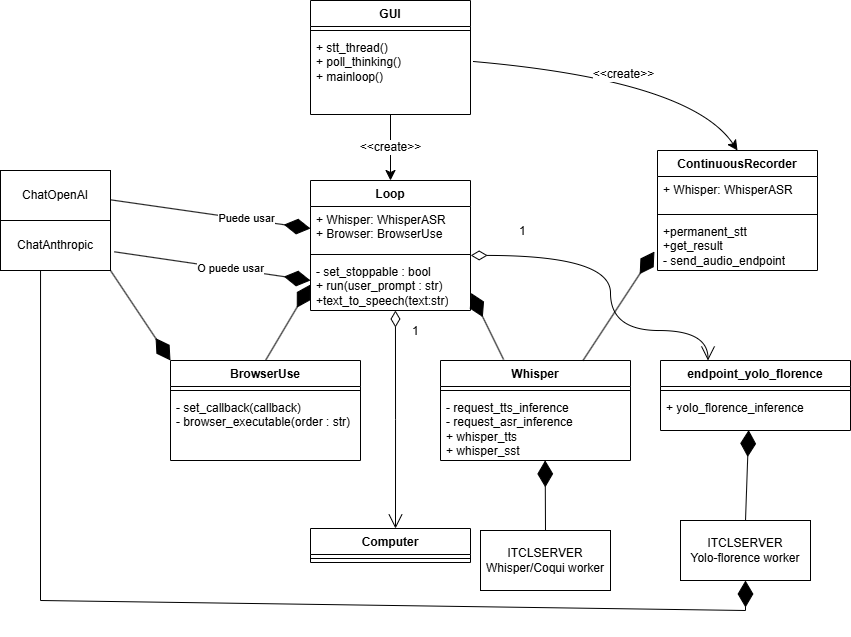
\includegraphics[scale=0.45]{img/Diagrama_clases.drawio.png}
  \caption{Diagrama de clases UML}
  \label{fig:UML}
\end{figure}

\subsection{Explicación de clases}
\begin{itemize}

    \item \textbf{GUI:} Representa la interfaz principal del programa, crea el Loop y hace uso de \texttt{ContinuousRecorder} para realizar inferencia continua sobre el audio recibido.

    \item \textbf{Loop:} La clase central del agente. \texttt{Loop} está compuesta por \texttt{BrowserUse} y \texttt{Whisper}, ya que necesita de ambas para cumplir su funcionalidad principal. 
    
    También incorpora una composición con las librerías de LangChain (\texttt{ChatOpenAI} o \texttt{ChatAnthropic}), siendo estas imprescindibles para el funcionamiento del sistema, aunque solo una puede estar activa en tiempo de ejecución.
    
    Adicionalmente, mantiene una dependencia con \texttt{endpoint-yolo-florence}, que permite la comprensión del contexto visual del entorno. Por último, \texttt{Loop} presenta una relación de agregación con el resto de herramientas de \texttt{Computer}, como escritura, movimiento de ratón, etc.

    \item \textbf{Whisper:} La clase \texttt{Whisper} tiene una composicion hacia \texttt{ContinuousRecorder} y \texttt{Loop}, ya que ambas dependen de ella para ejecutar funciones vitales. Estas funciones incluyen la transcripción continua del audio (STT) y la generación de archivos \texttt{.wav} con las respuestas del agente (TTS).
    
    Si bien la parte de TTS podría desacoplarse y gestionarse directamente desde \texttt{Whisper}, se ha optado por mantener esta responsabilidad dentro de \texttt{Loop}, dado que actúa como el núcleo del agente.
    
    Aunque esta implementación genera una composición fuerte, \texttt{Whisper} ha sido diseñada para realizar peticiones a un servidor externo del ITCL. Esto permite una cierta flexibilidad: para cambiar el modelo de inferencia (TTS/STT), solo sería necesario modificar el endpoint correspondiente dentro de \texttt{Whisper}, siempre y cuando el nuevo modelo siga utilizando los mismos formatos de entrada y salida.
    
    \item \textbf{BrowserUse:} Aunque no es estrictamente necesaria para el funcionamiento del agente, ya que algunas herramientas internas de \texttt{Computer} pueden cubrir parcialmente sus funciones, se ha optado por incluirla mediante composición dentro de \texttt{Loop}, ya que mejora considerablemente la precisión en las tareas de búsqueda.
    
    Cabe mencionar que \texttt{BrowserUse} depende completamente de \texttt{ChatAnthropic} para su funcionamiento, por lo que no puede operar sin esta.

    \item \textbf{ContinuousRecorder:} Aunque \texttt{GUI} no está compuesta directamente por esta clase ,debido a que existen funciones alternativas (actualmente desactivadas) para la transcripción, \texttt{ContinuousRecorder} representa un módulo importante dentro de la interfaz.
    
    Es responsable de la captura de audio y su conversión continua a texto sin interrupciones. Esta clase depende totalmente de \texttt{Whisper}, ya que sin ella no puede realizar las transcripciones.

    \item \textbf{endpoint-yolo-florence:} Al igual que \texttt{ContinuousRecorder}, este componente es esencial para ciertas funcionalidades de \texttt{Loop}, particularmente para la comprensión del contexto visual.
    
    No obstante, el agente puede seguir funcionando parcialmente sin él, motivo por el cual se ha modelado como una agregación y no como una composición directa desde \texttt{Loop}.

    \item \textbf{Computer:} Incluye herramientas auxiliares utilizadas por \texttt{Loop}, tales como el movimiento del ratón, escritura mediante teclado, y otras funcionalidades relacionadas con el control del sistema operativo.

    \item \textbf{ChatOpenAI / ChatAnthropic:} Son las interfaces que permiten interactuar con modelos de lenguaje a través de LangChain. Constituyen una parte fundamental del sistema, ya que sin ellas el agente no podría generar respuestas ni mantener una conversación.

    \item \textbf{ITCLSERVER Whisper / Coqui:} Corresponden a los modelos de inferencia TTS/STT alojados en los servidores del ITCL. Son utilizados por la clase \texttt{Whisper} para procesar el audio recibido (transcripción) o generar audio a partir de texto.
    
    \item \textbf{ITCLSERVER YOLO / Florence:} Contienen los modelos de visión por computador encargados de detectar objetos y generar una representación gráfica del entorno. La lógica actual de estos modelos está acoplada a \texttt{ChatAnthropic} para obtener descripciones semánticas, aunque esta parte podría desacoplarse fácilmente y ubicarse directamente dentro de \texttt{endpoint-yolo-florence}.
    
    Esto permitiría que el endpoint devuelva un diccionario de índices, coordenadas, descripciones y una imagen procesada ("yoleada"), facilitando así una mayor modularidad. Sin embargo, por motivos de simplicidad y comodidad, se ha mantenido la lógica actual en el worker.

\end{itemize}

\subsection{Diseño centrado en la clase Loop}
Durante el desarrollo del agente, se tomó la decisión de estructurar el sistema de forma que la clase \texttt{Loop} actuase como el núcleo central de la aplicación. Esta elección responde a la necesidad de contar con un componente que coordinara de forma ordenada todas las funcionalidades críticas del sistema: procesamiento de lenguaje natural, transformacion de audio a texto, percepción visual del entorno, interacción con herramientas del sistema operativo y uso de fuentes externas como navegadores.

\texttt{Loop} se encarga de realizar la ejecución del agente, controlando cuándo y cómo deben actuar los distintos módulos. Por esta razón, se le asignaron relaciones de composición con elementos esenciales como \texttt{Whisper} (para STT y TTS), \texttt{BrowserUse} (búsqueda en la web), y las librerías de LangChain (\texttt{ChatOpenAI} o \texttt{ChatAnthropic}), ya que su funcionamiento correcto depende directamente de estos para llevar a cabo su lógica y función principal.

Adicionalmente, \texttt{Loop} mantiene relaciones de agregación con componentes más secundarios, como los módulos de visión (\texttt{endpoint yolo-florence}) o las herramientas de \texttt{Computer} (teclado, ratón, etc.), permitiendo que estas puedan activadas o desactivadas sin comprometer la integridad del sistema.

Aunque esta centralización puede dar lugar a una clase con muchas responsabilidades, lo que en ingeniería del software se conoce como un "God Object", en este caso se justifica plenamente por el contexto del proyecto. Al tratarse de un agente que debe operar de manera autónoma y reactiva, resulta conveniente contar con un único punto de entrada que mantenga el control y secuenciación de los diferentes módulos.

Además, este diseño permite una clara separación entre el núcleo lógico del agente y sus módulos funcionales. Cada clase ha sido diseñada para tener responsabilidades bien delimitadas, permitiendo que su lógica interna se mantenga lo más independiente posible. Esta modularidad facilita la sustitución de componentes individuales (por ejemplo, cambiar el modelo de lenguaje o el motor de transcripción) sin necesidad de alterar el diseño general del sistema.

\subsubsection{Conclusion}
He priorizado un enfoque que combina centralización lógica en \texttt{Loop} con una arquitectura modular, en la que cada componente mantiene un alto grado de cohesión. Esta estructura no solo facilita el mantenimiento y la escalabilidad futura del proyecto, sino que también hace más clara su comprensión y evaluación.

\section{Diseño procedimental}

En este apartado describire la lógica del flujo de trabajo del sistema relacionado con las tareas principales de la aplicación.


\begin{enumerate}
\item La clase \texttt{GUI} inicia la ejecución del programa y lanza un bucle continuo gestionado por la clase \texttt{Loop} para inicializar el CUA.

\item \texttt{Loop} activa el contenedor de \texttt{Whisper}, que emplea \texttt{ContinuousRecorder} para comenzar la captura y transcripción continua de audio.

\item Cuando se detecta un prompt de voz, se valida la entrada y se encapsula como un prompt. En caso de hacer una introducción por teclado simplemente habría que escribir el prompt y enviarlo.

\item El prompt es analizado por el modelo LLM (a través de \texttt{ChatOpenAI} o \texttt{ChatAnthropic}) para extraer la intención del usuario.

\item Si el LLM determina que necesita información visual, se activa el endpoint \texttt{yolo-florence}, que genera una descripción semántica del entorno gráfico.

\item Si la tarea requiere datos externos, \texttt{BrowserUse} lanza una búsqueda web y filtra los resultados obtenidos.

\item Una vez recolectada toda la información necesaria (contexto visual, datos externos, historial, etc.), el agente genera una respuesta textual, que se muestra al usuario a través de la interfaz \texttt{GUI}.

\item En caso de ser necesario para cumplir la intención del usuario, el agente utilizaría herramientas incorporadas para conseguir el objetivo descrito por el usuario.

\item Opcionalmente, la respuesta puede ser vocalizada. Para ello, \texttt{Loop} reutiliza \texttt{Whisper} para convertir el texto en audio mediante TTS, el cual se reproduce automáticamente.

\item Finalmente, el agente queda de nuevo en espera de una nueva interacción, reiniciando el ciclo.
\end{enumerate}

A continuación se mostrara el diagrama de secuencia de todas las tareas mencionadas anteriormente.

\begin{figure}[h!]
  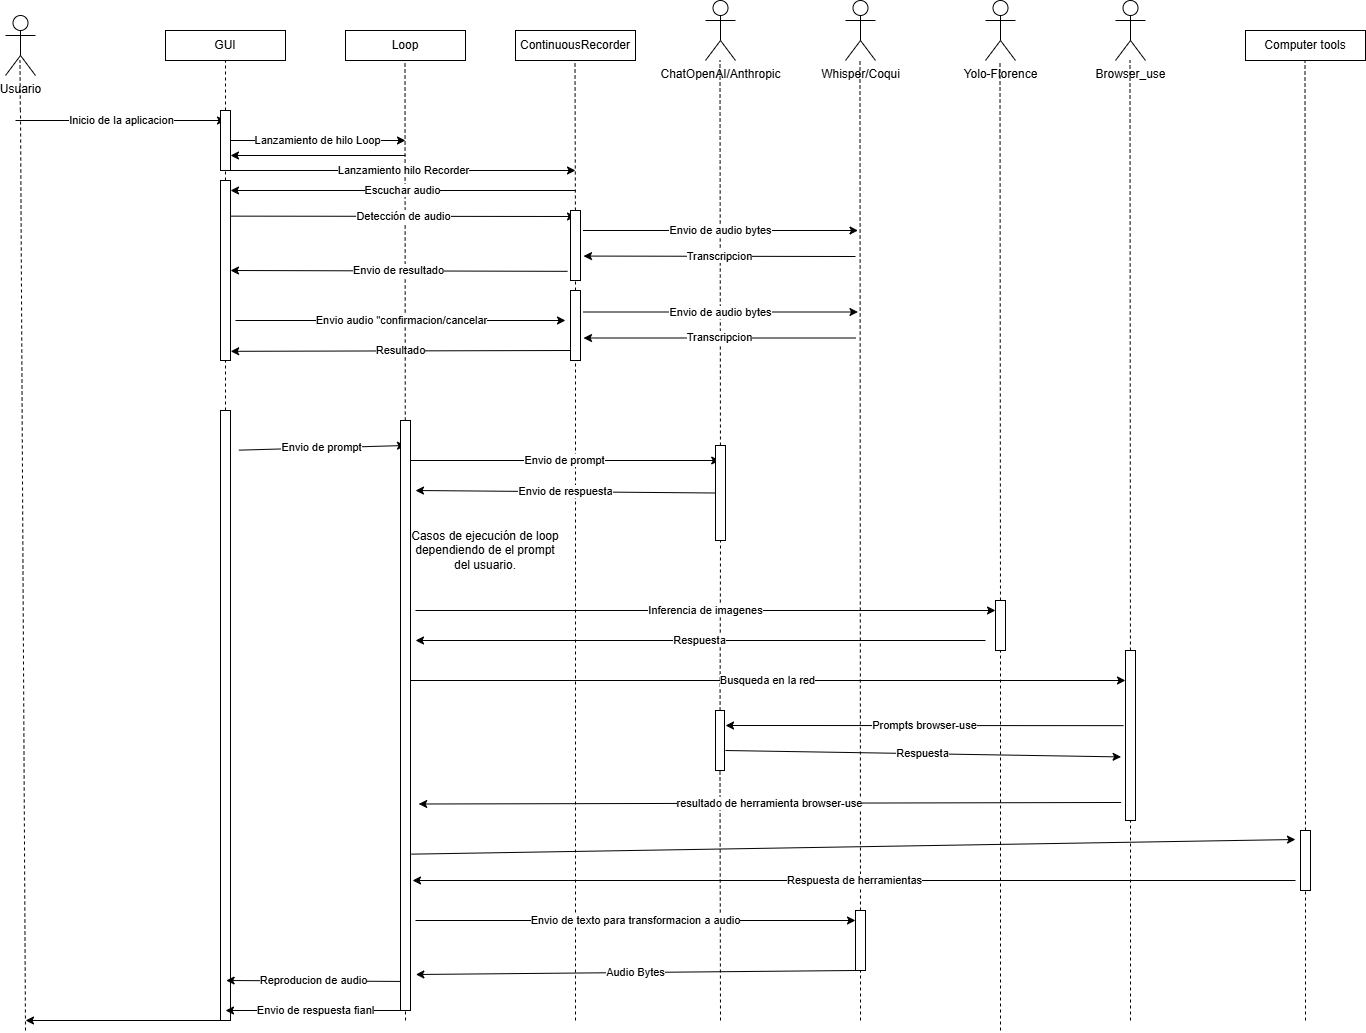
\includegraphics[scale=0.35]{img/Diagrama secuencia.drawio.png}
  \caption{Diagrama de secuencia de todas las tareas.}
  \label{fig:UML}
\end{figure}
\apendice{Documentación técnica de programación}

\section{Introducción}

\section{Datos tratados}


\section{Estructura de directorios}

\begin{itemize}
  \item \textbf{Raíz del proyecto (VACA/)}
  \begin{itemize}
    \item \texttt{main\_loop.py} -- Bucle principal del agente
    \item \texttt{gui.py} -- Interfaz gráfica en CTkinter
    \item \texttt{initializer.py} -- Inicialización del entorno
    \item \texttt{.env}, \texttt{pyproject.toml}, \texttt{README.md}
  \end{itemize}
  
  \item \textbf{CUA/} -- Módulo central del agente
  \begin{itemize}
    \item \texttt{cfg.py}, \texttt{\_\_init\_\_.py}
    \item \textbf{tools/}
    \begin{itemize}
      \item \texttt{class\_whisper.py}, \texttt{class\_browser\_use.py}, \texttt{computer.py}
      \item \texttt{endpoint\_yolo\_florence.py} -- Objetos de los modelos para instanciación y tools varias.
      \item \texttt{audio\_TTS.wav}, \texttt{output.wav} -- Generacion de TTS y STT
      \item \textbf{tmpcrops/} -- Capturas temporales para detección de elementos visuales
    \end{itemize}
    \item \textbf{util/} -- Funciones de soporte (configuración, rutas, logs)
  \end{itemize}

  \item \textbf{assets/} -- Material gráfico del proyecto
  \begin{itemize}
    \item Diagramas: \texttt{CUA FLOW.png}, \texttt{GUI\_inicial.png}, \texttt{resultado\_final.png}
    \item Pruebas visuales: \texttt{ejemplo\_original.jpeg}, \texttt{ejemplo\_yoloed.jpeg}
    \item Videos demostrativos: \texttt{cua\_example1.mp4}, \texttt{cua\_example2.mp4}
  \end{itemize}

  \item \textbf{tests/} -- Suite de pruebas del sistema
  \begin{itemize}
    \item \texttt{test\_001\_ScreenAssistant.py}, \texttt{test\_002\_Florence.py}, etc.
    \item \textbf{resources/}
    \begin{itemize}
      \item \textbf{generatedAudio/} -- Audios generados en pruebas
      \item \textbf{generatedimage/} -- Imágenes procesadas por los modelos
    \end{itemize}
  \end{itemize}

  \item \textbf{logs/} -- Registro de eventos y configuración
  \begin{itemize}
    \item \texttt{CUA.util.cfg\_base.log}
  \end{itemize}
\end{itemize}


\section{Manual del programador}

En esta sección elaborare una "visión" técnica para que cualquier otra persona que desee comprender, mantener o mejorar la aplicación VACA.

A continuación detallare los módulos clave y las dependendias principales del proyecto:

\begin{itemize}
    \item \textbf{Lenguaje de programación:} Python 3.12
    \item \textbf{Gestor de dependencias:} Poetry
    \item \textbf{Frameworks y librerías clave:}
    \begin{itemize}
        \item \texttt{openai, langchain-openai, langchain-anthropic,python-dotenv}
        \item \texttt{pyautogui, pillow,anthropic,langchain}
        \item \texttt{opencv-python, screeninfo, ultralytics,safetensors}
        \item \texttt{transformers,langchain-community,keyboard}
        \item \texttt{timm,einops,langgraph,logging}
        \item \texttt{pyaudio,wave,browser-use}
        \item \texttt{threaded}
    \end{itemize}
    \item \textbf{Estructura modular:}
    \begin{itemize}
        \item Módulo \texttt{CUA/}: lógica del agente, herramientas de audio y visión.
        \item \texttt{main\_loop.py}: orquestador del flujo principal.
        \item \texttt{gui.py}: interfaz visual del sistema.
        \item \texttt{initializer.py}: carga inicial para levantar modelos del servidor del ITCL.
    \end{itemize}
\end{itemize}

\subsection{Instrucciones para ejecución sin modelos dockerizados}

En caso de querer ejecutar la aplicación sin utilizar los modelos dockerizados para \texttt{Whisper}, \texttt{Coqui}, \texttt{Florence} o \texttt{YOLO}, se proporciona en el repositorio de GitHub el contenedor Docker correspondiente al modelo \texttt{Florence-YOLO}, facilitando así su despliegue local. Para ello, únicamente sería necesario adaptar los endpoints a la configuración local deseada.

Respecto a los modelos \texttt{Whisper} y \texttt{Coqui}, no se incluyen directamente en el proyecto debido a motivos dep privacidad. Sin embargo, ambos modelos son de código abierto y están disponibles en los siguientes enlaces:

\begin{itemize}

\item \textbf{Coqui XTTS-v2}\cite{coquiXTTSv2}
\item \textbf{OpenAI Whisper Large v3}\cite{openaiWhisperV3}
\end{itemize}

Para ejecutar el sistema sin estos modelos, se recomienda desactivar el módulo de TTS (activado por defecto) y también el hilo de transcripción continua (STT) que se lanza desde la clase \texttt{GUI}. Esta configuración permitirá el uso parcial del agente sin necesidad de contar con los modelos de voz en funcionamiento, manteniendo otras funcionalidades operativas.





\section{Compilación, instalación y ejecución del proyecto}

En esta sección se describen los pasos necesarios para compilar, instalar y ejecutar correctamente la aplicación \textbf{VACA}.

\subsection{Descarga del programa desde GitHub}

El código del proyecto se encuentra disponible en el repositorio personal del alumno. Se recomienda descargar la última versión publicada en la sección de releases del repositorio.\cite{VACARepo}

\subsection{Instalación de los programas necesarios e inicialización}

Para la correcta ejecución del proyecto, se deben seguir los siguientes pasos:

\begin{enumerate}
    \item Instalar un entorno de desarrollo para Python. En este caso se ha utilizado Visual Studio Code, aunque puede utilizarse cualquier otro compatible.
    \item Instalar Python en su versión 3.12. \cite{python312}
    
    \item Instalar un gestor de entornos virtuales compatible con archivos \texttt{pyproject.toml}. En este proyecto se ha utilizado \textbf{Poetry}\cite{poetryDocs}.
    
    \item Crear un nuevo entorno virtual y utilizar el archivo \texttt{pyproject.toml} del repositorio para importar automáticamente todas las librerías necesarias.
    
    \item Una vez finalizada la instalación de dependencias, se puede ejecutar el archivo \texttt{gui.py}, el cual lanza la interfaz principal del programa.
\end{enumerate}

\subsection{Recomendaciones de uso}

Se recomienda encarecidamente utilizar un sistema con doble monitor, ya que la aplicación trabaja principalmente sobre el monitor configurado como principal, y requiere visibilidad total del entorno gráfico para su funcionamiento correcto.

\section{Pruebas del sistema}

El sistema fue sometido a diversas pruebas con el objetivo de garantizar su correcto funcionamiento en distintos contextos de uso.

Dado que \textbf{VACA} se basa en el uso de modelos de lenguaje de gran escala (LLM) y controla el entorno operativo del usuario, muchas de las pruebas fueron realizadas de forma manual. Esto se debe a que, por la naturaleza del sistema, cualquier ejecución fuera de control podría requerir intervención humana para ser detenida o corregida.

\subsection{Pruebas automatizadas}

Se implementó una batería de pruebas unitarias y funcionales que puede encontrarse en la carpeta \texttt{test} del repositorio del proyecto. Estas pruebas tienen como objetivo verificar el correcto funcionamiento individual de los distintos módulos que componen el sistema.

Para ejecutar todas las pruebas, basta con utilizar el siguiente comando en el entorno del proyecto:

\texttt{pytests \@master\_test.txt}

Este comando lanza la ejecución de todos los casos definidos de manera estructurada.

Adicionalmente, se valoró la posibilidad de integrar la aplicación en un entorno de evaluación tipo \textit{benchmark} con el fin de analizar su rendimiento de forma más rigurosa. Sin embargo, debido a que se trata de un agente de "reciente" y que funciona exclusivamente sobre el sistema operativo Windows, no existen muchas opciones disponibles.

La única alternativa identificada fue el entorno de evaluación \textbf{Windows Agent Arena} \cite{Bonatti2024WindowsAgentArena}. No obstante, su integración se descartó en esta fase del proyecto debido a la falta de tiempo y la complejidad técnica para su puesta en marcha, quedando como posible mejora a implementar en el futuro.

\apendice{Documentación de usuario}

\section{Introducción}

Esta sección tiene como objetivo proporcionar a los usuarios finales una guía clara y concisa sobre el uso de la aplicación \textbf{VACA} (Voice Assisted Computer Accessibility). Se detallan los requisitos necesarios, el proceso de instalación, y un manual de uso básico para facilitar su adopción.

\section{Requisitos de usuarios}

\subsection{Requisitos del sistema}

Para garantizar el correcto funcionamiento de la aplicación \textbf{VACA}, es necesario cumplir con los siguientes requisitos mínimos, diferenciados entre componentes de software y hardware.

\subsubsection{Requisitos de software}

\begin{itemize}
    \item \textbf{Sistema operativo:} Microsoft Windows 10 o superior.
    \item \textbf{Versión de Python:} Python 3.12 instalado correctamente en el sistema.
    \item \textbf{Dependencias:} Todas las bibliotecas necesarias especificadas en el archivo \texttt{pyproject.toml}, las cuales deben instalarse mediante un gestor compatible como \textbf{Poetry}.
\end{itemize}

\subsubsection{Requisitos de hardware}

\begin{itemize}
    \item \textbf{Micrófono:} Necesario para utilizar las funcionalidades de reconocimiento de voz (STT).
    \item \textbf{Altavoces o salida de audio:} Requeridos para escuchar las respuestas generadas por el sistema mediante síntesis de voz (TTS).
    \item \textbf{Pantallas:} Se recomienda disponer de una configuración de doble monitor. Idealmente, la pantalla principal debe estar situada en el centro y la secundaria a la derecha. Aunque no es estrictamente obligatorio, esta disposición facilita la interacción con el sistema, permitiendo que el usuario visualice el funcionamiento de \textbf{VACA} en la pantalla secundaria, mientras el programa opera sobre la principal.
\end{itemize}

\section{Instalación}
El procedimiento de instalación está pensado para usuarios con conocimientos básicos de informática. Los pasos a seguir son:

\begin{enumerate}
    \item Descargar la última versión de la aplicación desde el repositorio oficial en GitHub: \url{https://github.com/VictorManuelMG/TFGGII_VACA}. \cite{VACARepo}
    \item Instalar \textbf{Python 3.12} desde \url{https://www.python.org/downloads/release/python-3120/}.\cite{python312}
    \item Instalar \textbf{Poetry} como gestor de entornos virtuales, siguiendo la documentación oficial: \url{https://python-poetry.org/docs/}.\cite{poetryDocs}
    \item Definir en \texttt{.env.example} las APIs necesarias.
    \item Abrir una terminal en la carpeta del proyecto y ejecutar el comando \texttt{poetry install} para instalar las dependencias.
    \item Iniciar la aplicación ejecutando el archivo \texttt{gui.py} con el comando \texttt{poetry run python gui.py}.
\end{enumerate}

\section{Manual del usuario}

El uso de la aplicación \textbf{VACA} ha sido diseñado para ser intuitivo. Todas las operaciones se realizan desde la interfaz gráfica integrada que se muestra a continuación:

\begin{figure}[h!]
\centering
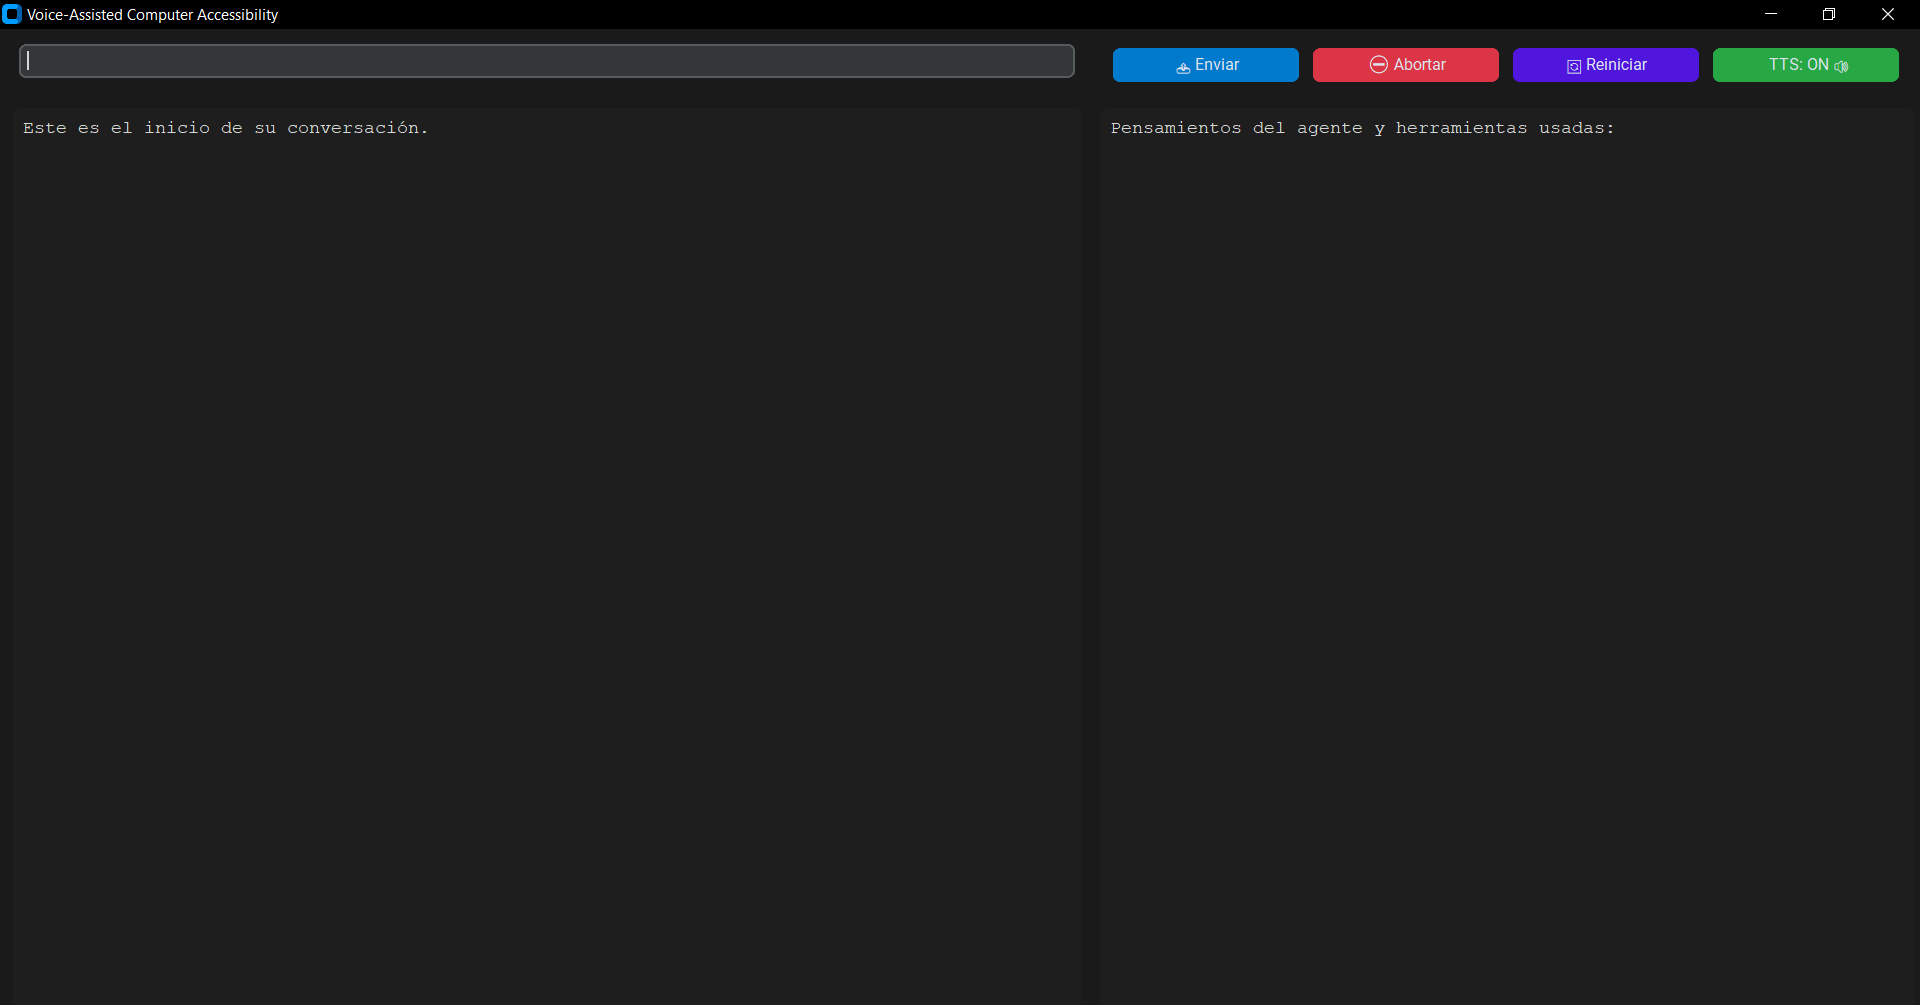
\includegraphics[scale=0.35]{img/interfaz.png}
\caption{Interfaz de usuario.}
\label{fig:manual_interfaz}
\end{figure}

Como puede observarse, la interfaz cuenta con un cuadro de entrada de texto y varios botones con distintas acciones situados en los laterales. El sistema admite entrada de comandos tanto por texto como por voz.

\subsection{Entrada por voz}

\begin{figure}[h!]
\centering
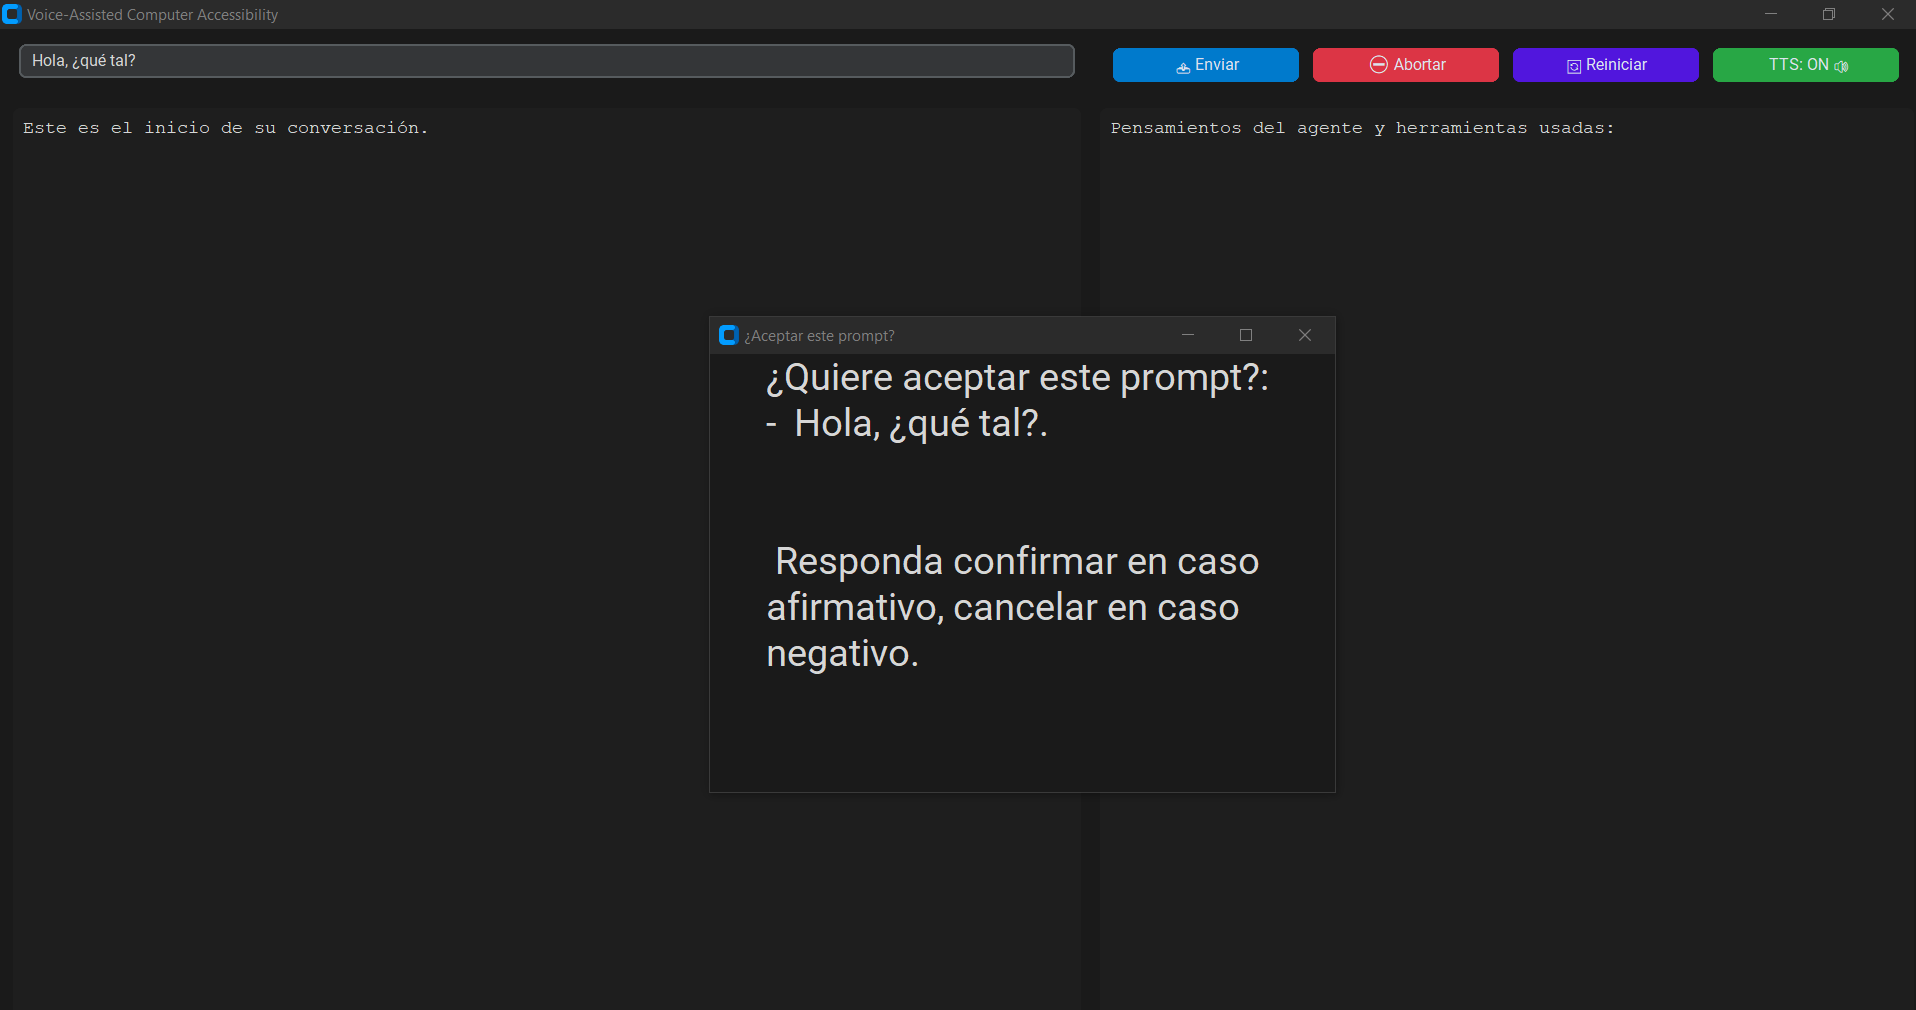
\includegraphics[scale=0.35]{img/input_voz.png}
\caption{Entrada de un prompt mediante voz.}
\label{fig:input_voz}
\end{figure}

Para utilizar esta funcionalidad, basta con hablar al micrófono tras iniciar el programa. Una vez que el comando de voz ha sido capturado y confirmado, el sistema procede automáticamente a procesar la petición del usuario.

\begin{figure}[h!]
\centering
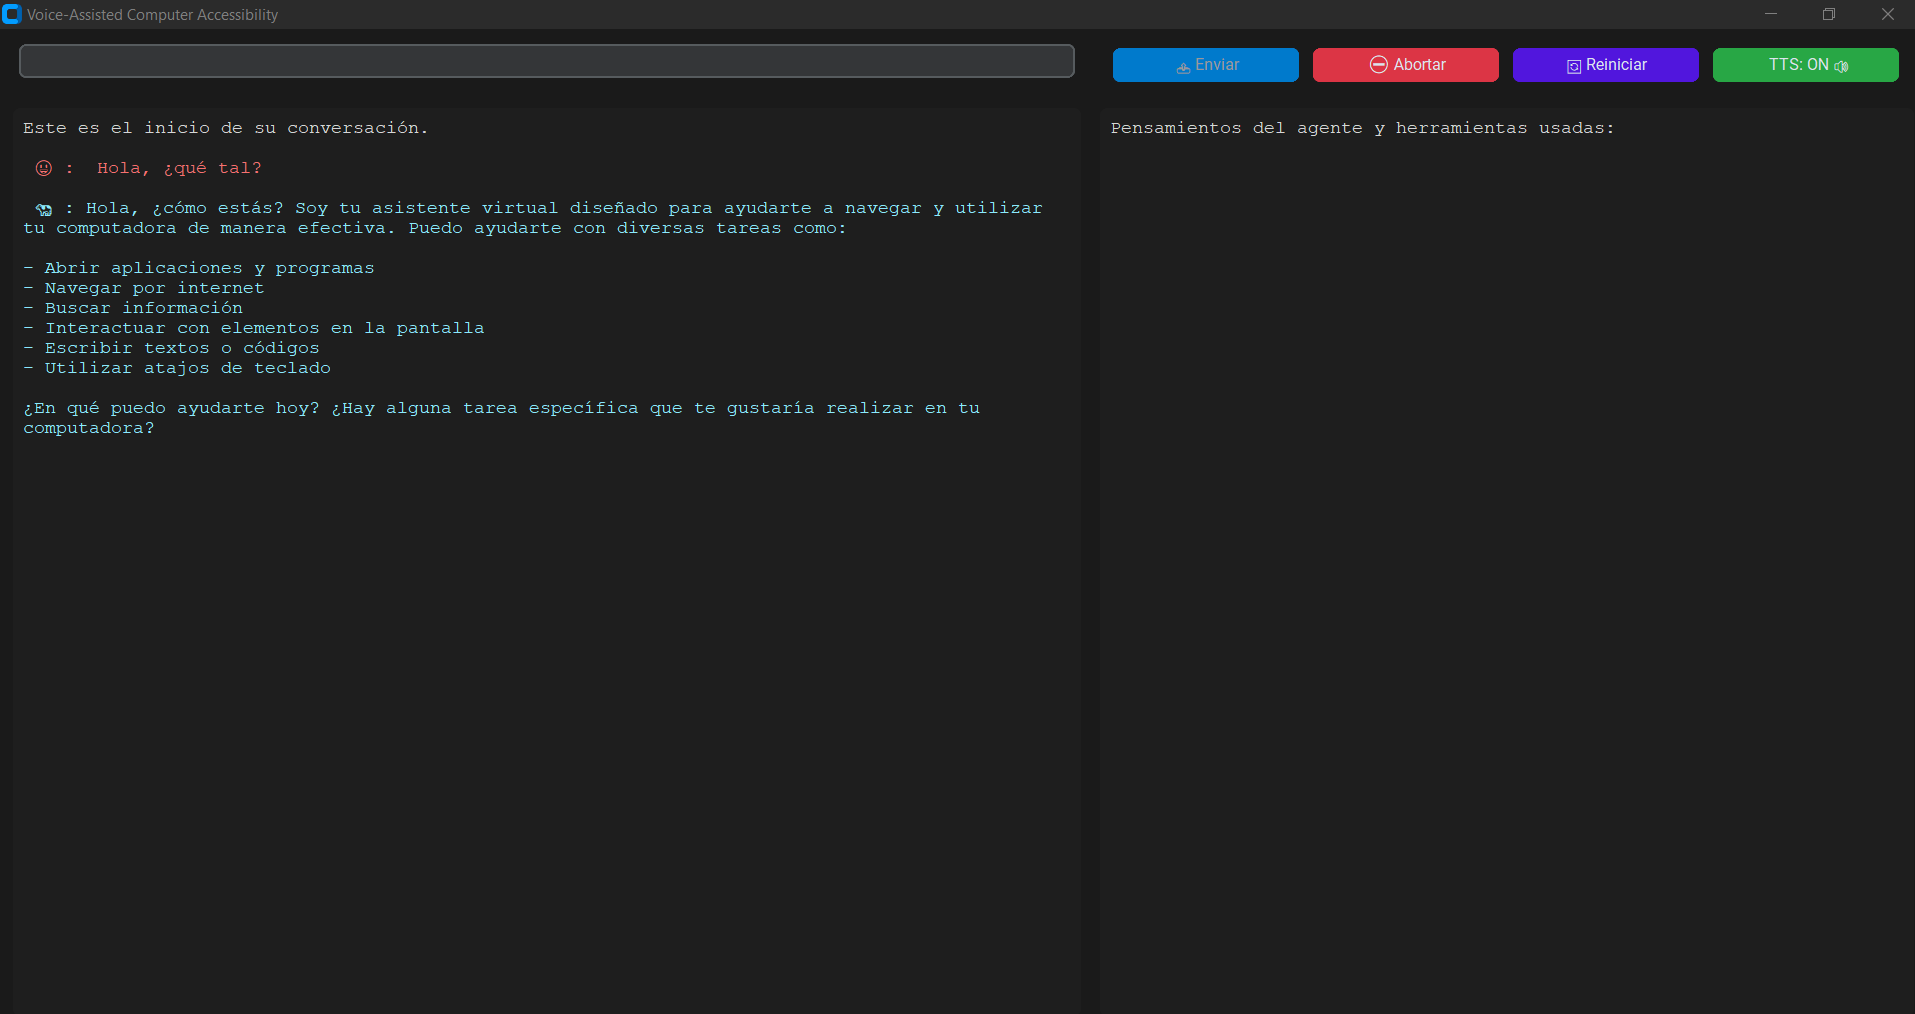
\includegraphics[scale=0.35]{img/Output_voz.png}
\caption{Respuesta generada tras la entrada por voz.}
\label{fig:output_voz}
\end{figure}

Como se muestra en la imagen anterior, tras procesar el prompt, el sistema devuelve una respuesta visual (y opcionalmente también por voz, si el TTS está activado).

\subsection{Visualización de pensamientos del agente}

Además de los resultados visibles de cada acción, el sistema muestra en tiempo real los \textbf{pensamientos del agente}, es decir, los razonamientos internos que realiza al ejecutar determinadas tareas, como la búsqueda de información o el análisis del entorno.

\begin{figure}[h!]
\centering
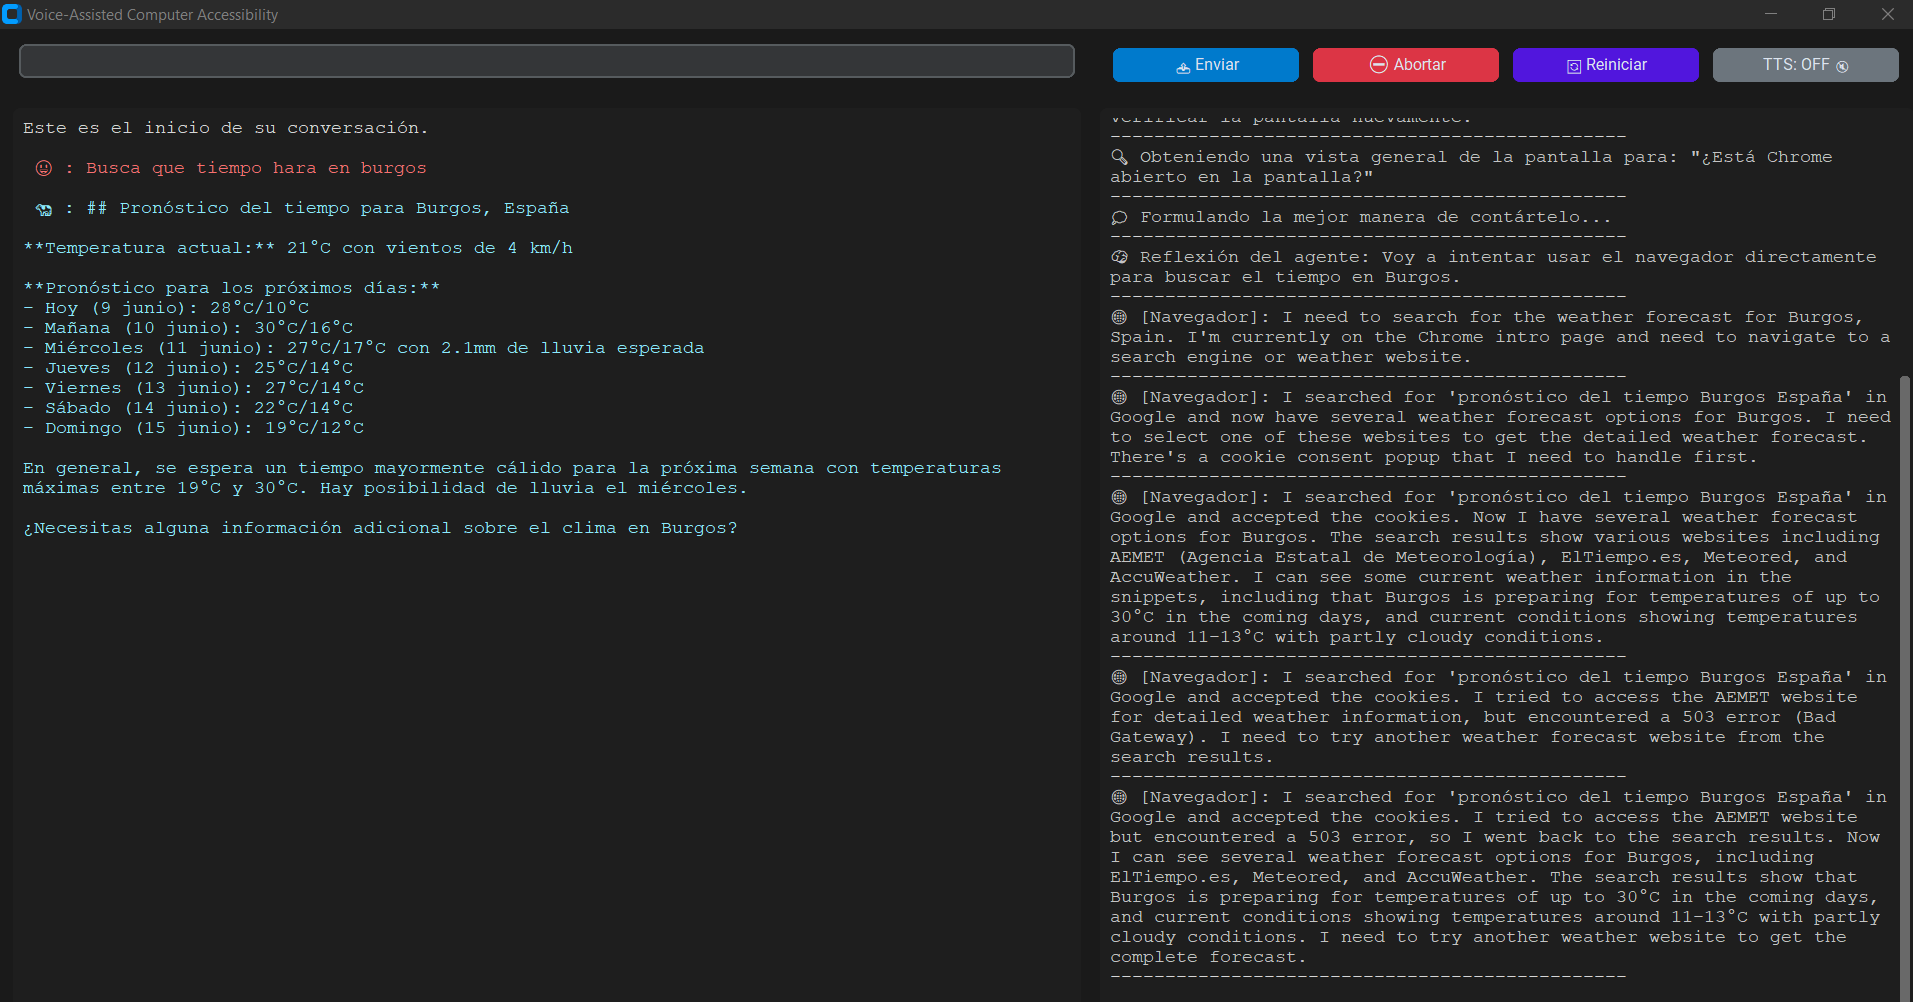
\includegraphics[scale=0.35]{img/Output_search.png}
\caption{Ejemplo de razonamiento mostrado durante una búsqueda en internet.}
\label{fig:output_search}
\end{figure}

Esta funcionalidad permite al usuario comprender mejor qué está haciendo el sistema en cada momento y seguir su lógica de actuación.

\subsection{Recomendaciones de uso}

Se recomienda encarecidamente utilizar un micrófono de buena calidad para garantizar una correcta detección de voz. En caso contrario, podrían producirse errores de reconocimiento. Actualmente, la interfaz no incluye opciones de configuración avanzada del audio, por lo que ajustes como la sensibilidad del micrófono, la ganancia o la amplificación deberán realizarse directamente desde la configuración del sistema operativo.

En futuras versiones se contempla incluir un apartado de configuración accesible desde la propia interfaz para facilitar esta tarea al usuario.
\apendice{Anexo de sostenibilización curricular}

\section{Introducción}

Este anexo tiene como objetivo hacer una reflexión personal sobre cómo se han abordado temas de sostenibilidad a lo largo del desarrollo de este Trabajo de Fin de Grado (TFG). A través del proyecto \textbf{VACA} (Voice Assisted Computer Accessibility), he podido trabajar no solo con herramientas técnicas, sino también con ideas relacionadas con la accesibilidad, la inclusión, el uso responsable de la tecnología y el impacto que puede tener un software en el entorno y en las personas.

\section{Contribución del TFG a la inclusión social}

Desde el principio, uno de los objetivos principales del proyecto fue crear una herramienta que pudiera ayudar a personas con movilidad reducida a interactuar con su ordenador de forma más sencilla. \textbf{VACA} permite controlar el equipo mediante comandos de voz, algo que puede marcar la diferencia para muchos usuarios que no pueden utilizar el teclado o el ratón con normalidad.

Esto conecta directamente con la idea de reducir desigualdades, tal como plantea el Objetivo de Desarrollo Sostenible (ODS) número 10 de la ONU. Me parece importante que desde la informática se puedan proponer soluciones que tengan un impacto positivo en la vida de la gente, especialmente en colectivos que suelen quedar fuera del foco tecnológico.

\section{Sostenibilidad tecnológica y uso de software libre}

Durante todo el desarrollo he apostado por el uso de herramientas y modelos de código abierto como Whisper, Coqui o Florence. Además de ser gratuitos, estos recursos están disponibles para toda la comunidad, lo que permite que otras personas puedan aprovecharlos, mejorarlos o adaptarlos a sus propios proyectos.

Trabajar con software libre me ha hecho más consciente del valor de compartir el conocimiento, y también de cómo esto ayuda a reducir barreras económicas. No depender de soluciones cerradas o de pago también puede ser una forma de hacer la tecnología más accesible para más gente, y eso encaja perfectamente con la idea de sostenibilidad social y económica.

\section{Impacto ambiental y decisiones técnicas}

Aunque muchas veces no lo pensemos, el software también tiene un impacto ambiental. Elegir si un modelo se ejecuta en local o en la nube puede influir en el consumo energético. En mi caso, he intentado que la mayoría de procesos puedan hacerse de forma local, sin necesidad de servidores externos. Esto no solo hace que el programa sea más rápido y autónomo, sino que también evita depender de infraestructuras que consumen muchos recursos.

También he intentado que el sistema no esté constantemente ejecutando procesos pesados si no son necesarios, lo que ayuda a optimizar el rendimiento y reducir el gasto de energía.

\section{Competencias de sostenibilidad adquiridas}

Durante el proyecto he aprendido muchas cosas, no solo técnicas, sino también relacionadas con la sostenibilidad. Por ejemplo, ahora tengo más claro que pensar en la accesibilidad no es solo un añadido, sino algo que debería formar parte del diseño desde el principio.

También he desarrollado una mirada más crítica a la hora de tomar decisiones técnicas. Ya que no se trata solo de incluir modelos sin gestión propia, sino también de que implicaría usar dicho modelo, si es abierto, si deja huella en internet, etc.

Por último, he podido ver cómo la informática puede ser una herramienta útil para cambiar cosas en el mundo real. A veces damos por hecho que los proyectos técnicos solo sirven para resolver problemas funcionales, pero también pueden tener un impacto social muy potente.

\section{Conclusión}

Este TFG me ha ayudado a tomar conciencia de cómo el desarrollo de software puede (y debería) hacerse teniendo en cuenta aspectos éticos y sostenibles. A lo largo del trabajo he intentado aplicar este enfoque en lo que estaba a mi alcance, y me ha motivado a seguir haciéndolo en el futuro.

Mi intención es seguir trabajando con esta mentalidad en los proyectos que vengan, combinando lo técnico con lo humano. Creo que la informática tiene un gran potencial para mejorar la vida de las personas, y que es responsabilidad nuestra como desarrolladores usar ese potencial de forma responsable y consciente.

En definitiva, este proyecto ha sido mucho más que una práctica técnica: me ha permitido abrir los ojos a un enfoque más completo y comprometido con la sociedad.


\bibliographystyle{plain}
\bibliography{bibliografiaAnexos}

\end{document}